\documentclass[final]{beamer} % beamer 3.10: do NOT use option hyperref={pdfpagelabels=false}!

%\documentclass[final,hyperref={pdfpagelabels=false}]{beamer} % beamer 3.07: get rid of beamer warnings


\renewcommand*\oldstylenums[1]{{\firaoldstyle #1}}

\mode<presentation>{\usetheme{dsmanchester}}


% Put any other packages or custom macros in here:
\PassOptionsToPackage{main=english}{babel}
\usepackage[english]{babel}
\usepackage[utf8]{inputenc}		% Codificacao do documento (convers\~{a}o autom\'{a}tica dos acentos)

\usepackage[sfdefault]{FiraSans} %% option 'sfdefault' activates Fira Sans as the default text font
%\usepackage{newtxsf}
\usepackage[T1]{fontenc}


\usepackage{mathtools}
\usepackage{bm}
\usepackage{cleveref} %cref, Cref
\usepackage{microtype} %aligning and stuff
\usepackage{exscale} %integral sign in poster
\usepackage{tikz}
\usepackage{mdframed}
\usetikzlibrary{calc}

% Portrait, A0 poster. Set scale as desired, but 1.3 gives easily readable text when printed.
\usepackage[orientation=portrait, size=custom, scale=1.3,width=91.44,height=152.4]{beamerposter}
% Set height of page for use in arranging text boxes, after accounting for
% heading, footer etc. This is a bit of a hack, ideally latex should figure
% this out for itself!
% \usepackage{geometry}
% \geometry{paperwidth=3ft, paperheight=5ft}
\newlength{\columnheight}
%133cm is all that remains
\setlength{\columnheight}{130cm}


\pdfstringdefDisableCommands{%
  \def\\{ }%
  \def\vspace{0.3em}{ }%
}

\newcommand{\hcurl}[1]{H (curl;#1)}
\newcommand{\hzcurl}[1]{H_0(curl;#1)}
\newcommand{\hone}[1]{H^1(#1)}
\newcommand{\hmspace}[1]{H^m(#1)}
\newcommand{\hzone}[1]{H^1_0(#1)}
\newcommand{\testhcurl}[0]{\bm{\varphi}}
\newcommand{\testhone}[0]{\varphi}
\newcommand{\pkspace}[2][k]{\mathbb{P}_{#1}(#2)}
\newcommand{\pkhomospace}[2][k]{\sim{\mathbb{P}}_{#1}(#2)}
\DeclareMathOperator{\curlop}{\nabla \times}
\DeclareMathOperator{\divop}{\nabla \cdot}
\DeclareMathOperator{\gradop}{\nabla}
\DeclareMathOperator{\curlopt}{\nabla_t \times}
\DeclareMathOperator{\divopt}{\nabla_t \cdot}
\DeclareMathOperator{\gradopt}{\nabla_t}

% Define the header information
\title{DEVELOPMENT OF HIGH-ORDER\\ \vspace{0.3em} \texorpdfstring{$\hcurl{\Omega}$}{H(CURL,OMEGA)}-CONFORMING APPROXIMATION SPACES FOR PHOTONIC WAVEGUIDE ANALYSIS}
% \title{Title \\ \vspace{0.3em} second line of title}
\author{Francisco T. Orlandini\texorpdfstring{\textsuperscript{1}}{ }, Hugo E. H. Figueroa\texorpdfstring{\textsuperscript{1}}{ } and Philippe R. B. Devloo\texorpdfstring{\textsuperscript{2}}{ }}
\institute{\texorpdfstring{\textsuperscript{1}}{ }School of Electrical and Computer Engineering, University of Campinas, Campinas-SP 13083-852, Brazil\\
\texorpdfstring{\textsuperscript{2}}{ }School of Civil Engineering, Architecture and Urban Design, University of Campinas, Campinas-SP 13083-852, Brazil}%

% Now start the actual poster
\begin{document}

% Header is automatically generated from the command defined in the theme
% file, the information above and the logos in the logo folder.


% Start of the body:
\begin{frame}
  \begin{columns}

    %% Left column:
    %% ============================================================
    \begin{column}{0.45\textwidth}

      % For some reason we need parbox to get it to arrange the boxes
      % with evenly spaced gaps
      \parbox[t][\columnheight]{\textwidth}{

        \vfill % vfill between every block so that everything is
               % automatically nicely spaced out.

        \begin{block}{ABSTRACT}
          \begin{itshape}   % italic abstract
             The advances in the fabrication of photonic waveguides in the past twenty years have led the scientific community to seek for numerical methods that could assist in the process of design of such devices. The design photonic waveguides often require relative errors of $10^{-14}$ on the dispersion parameters. In this context, a hierarchical strategy for constructing $\hcurl{\Omega}$-conforming elements is introduced, for application in a Finite Element Method (FEM) scheme for modal analysis of electromagnetic waveguides. The hierarchical $\hcurl{\Omega}$-conforming elements are used for the transversal component of the electric field, coupled with scalar $\hone{\Omega}$ elements for its longitudinal component. The Nédélec elements of the first kind were chosen for this work, and the ease of integration with \emph{p}-adaptivity schemes motivated the hierarchical construction of the FE basis. The scheme is assessed by means of the analysis of well-known waveguides. As a real-world scenario, the modal analysis of a Photonic Crystal Fiber illustrates the accuracy and the generalized eigenvalue problem size when dealing with a design process requiring high precision on the dispersion parameters.
            \end{itshape}
        \end{block}

        \vfill
        \begin{block}{\boxnumber FEM FORMULATION}
        Find non-trivial $\left(\beta^2,{e_t}, {e_z}\right) \in (\mathbb{C} \times [\mathbb{C}]^N \times [\mathbb{C}]^M)$ such that:
\begin{equation}\label{eq:fem-discretized-form}
  \begin{bmatrix}
    A_{tt} & 0 \\
    0      & 0
  \end{bmatrix}
  \begin{Bmatrix}
    e_t \\
    e_z
  \end{Bmatrix}
  = - \beta ^2
  \begin{bmatrix}
    B_{tt} & B_{tz} \\
    B_{zt} & B_{zz}
  \end{bmatrix}
  \begin{Bmatrix}
    e_t \\
    e_z
  \end{Bmatrix}
  \text{,}
\end{equation}
and the matrices are defined as:
\begin{align}
  [A_{tt}]_{ij} &= \int_{\Omega}
  \left[
  \mu_{zz}^{-1}\left( \curlopt \bm{\varphi}_i \right) \cdot
  \left( \curlopt \bm{\varphi}_j \right)
  - k_0^2 \bm{\epsilon}_{xy} \bm{\varphi}_i\cdot \bm{\varphi}_j\right] d\Omega\text{,}\label{eq:fem-mat-1}\\
  [B_{tt}]_{ij} &= \int_{\Omega}  \bm{\mu}_{xy^S}^{-1}\bm{\varphi}_i  \cdot
  \bm{\varphi}_j\, d\Omega\text{,}\label{eq:fem-mat-2}\\
  [B_{tz}]_{ij} &= \int_{\Omega}  \bm{\mu}_{xy^S}^{-1}\bm{\varphi}_i  \cdot
  \gradopt \testhone_j\, d\Omega\text{,}\label{eq:fem-mat-3}\\
  [B_{zt}]_{ij} &= \int_{\Omega}  \bm{\mu}_{xy^S}^{-1}\gradopt \testhone_i  \cdot
  \bm{\varphi}_j
  \, d\Omega\text{,}\label{eq:fem-mat-4}\\
  [B_{zz}]_{ij} &= \int_{\Omega}
  \left[
  \bm{\mu}_r^{-1}\gradopt \testhone_i  \cdot
  \gradopt \testhone_j
  - k_0^2 \epsilon_{zz} \testhone_i \testhone_j\right] d\Omega\text{.}\label{eq:fem-mat-5}
\end{align}
        \end{block}
        \begin{block}{\boxnumber EFFECTS OF GEOMETRICAL REPRESENTATION}
        \begin{figure}[ht]
            \centering
            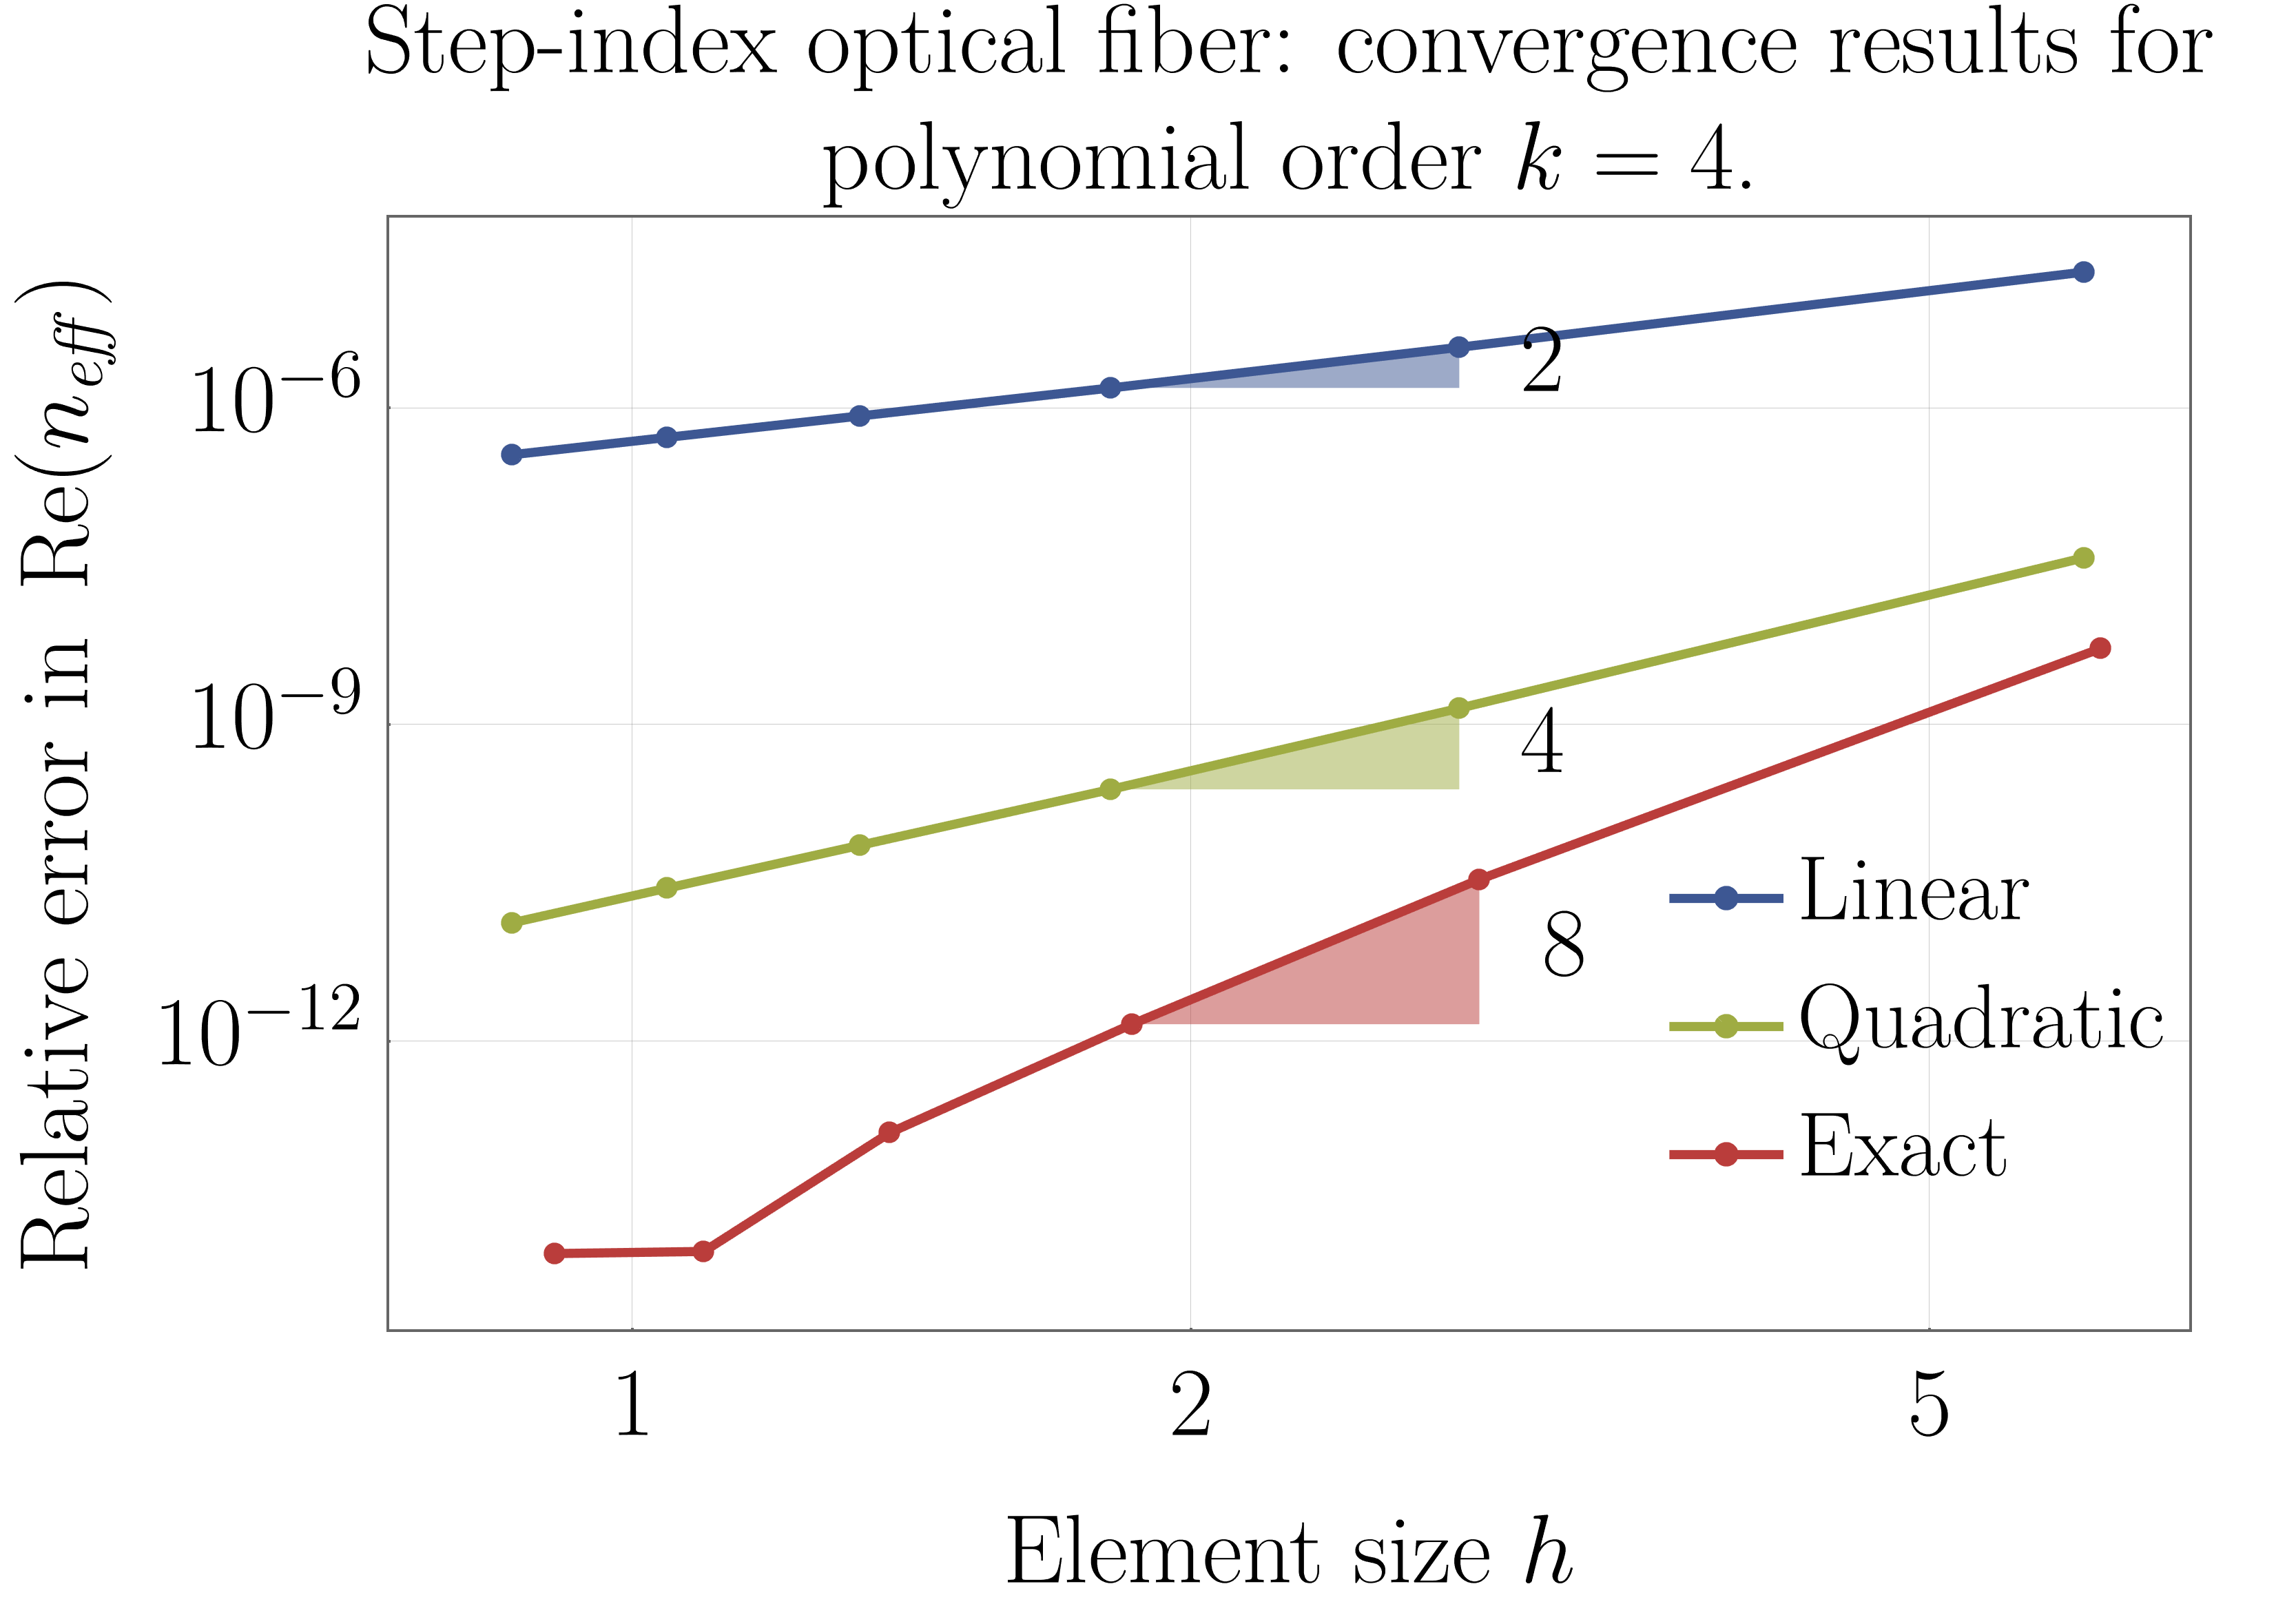
\includegraphics[width=0.8\linewidth]{images/convergenceRates_k4_poster.png}
            \caption{BlaBlabla}
            \label{fig:test}
        \end{figure}
        
        On a last note regarding implementation choices, there is the matter of \emph{scaling}. The electromagnetic quantities present in a computation of the generalized eigenvalue problem obtained in \Cref{eq:fem-discretized-form} vary widely in magnitude. The $k_0$ factor, in the context of photonics, can easily reach orders of magnitude around $10^6$, while the cross-sectional area of waveguides such as optical fibers can be as small as $10^{-14}m^2$. In order to reduce the floating-point errors, \Cref{eq:fem-discretized-form} was scaled by the factor $k_0$, so the resulting eigenvalue of \Cref{eq:fem-discretized-form} is now $-n_{eff}^2$, given that the \emph{effective refractive index} is calculated by $n_{eff} = \beta/k_0$.
        \begin{figure}[hb]
        	\begin{mdframed}[backgroundcolor=bggrey]
        		Ez \hfill Et
        		
	            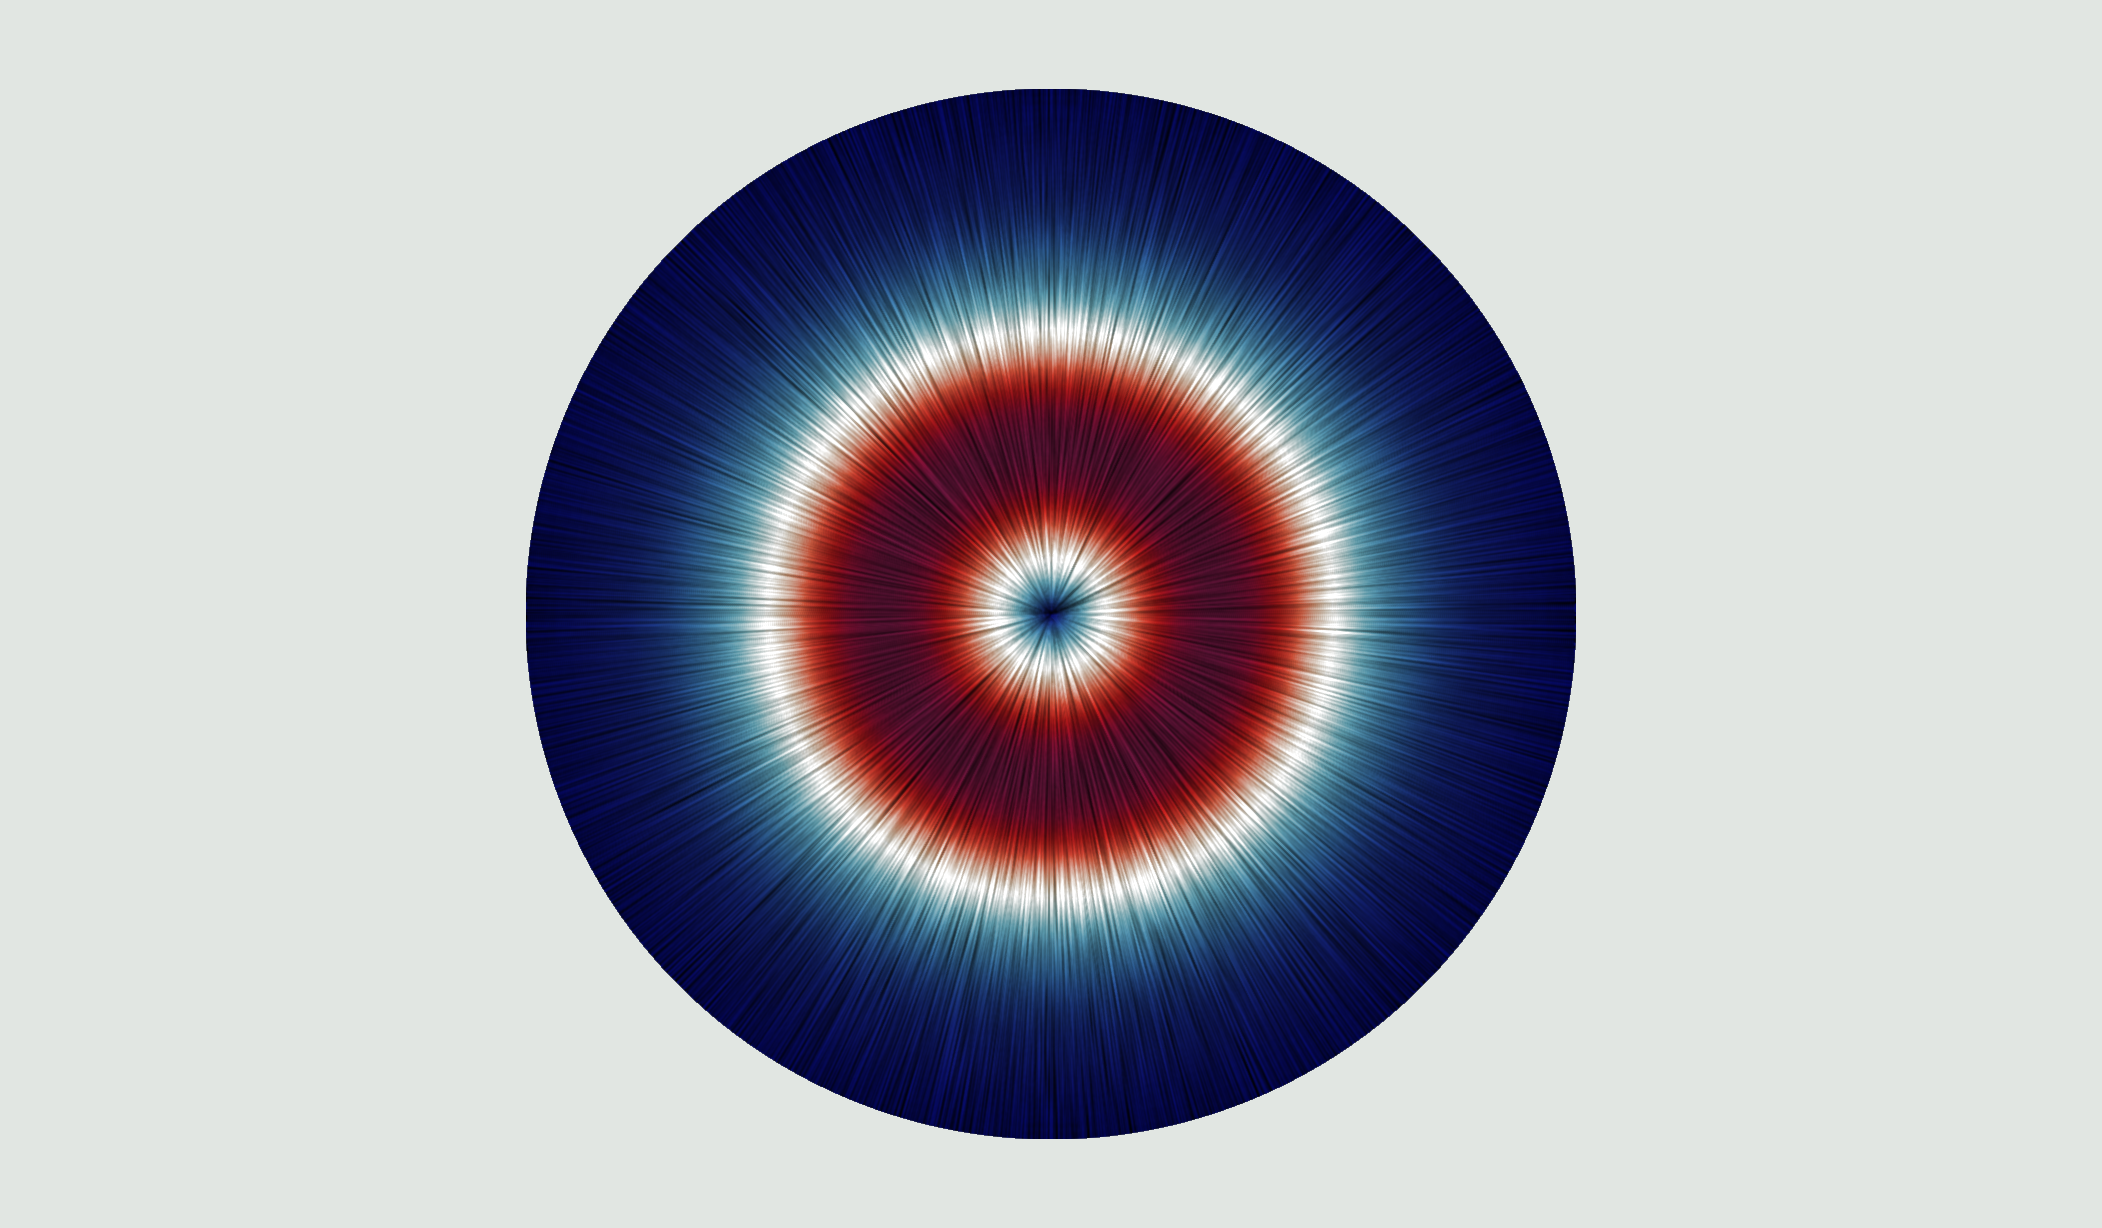
\includegraphics[width=0.49\textwidth]{images/et2posterStepFiber.png}%
	            \hspace{0.01\textwidth}%
	            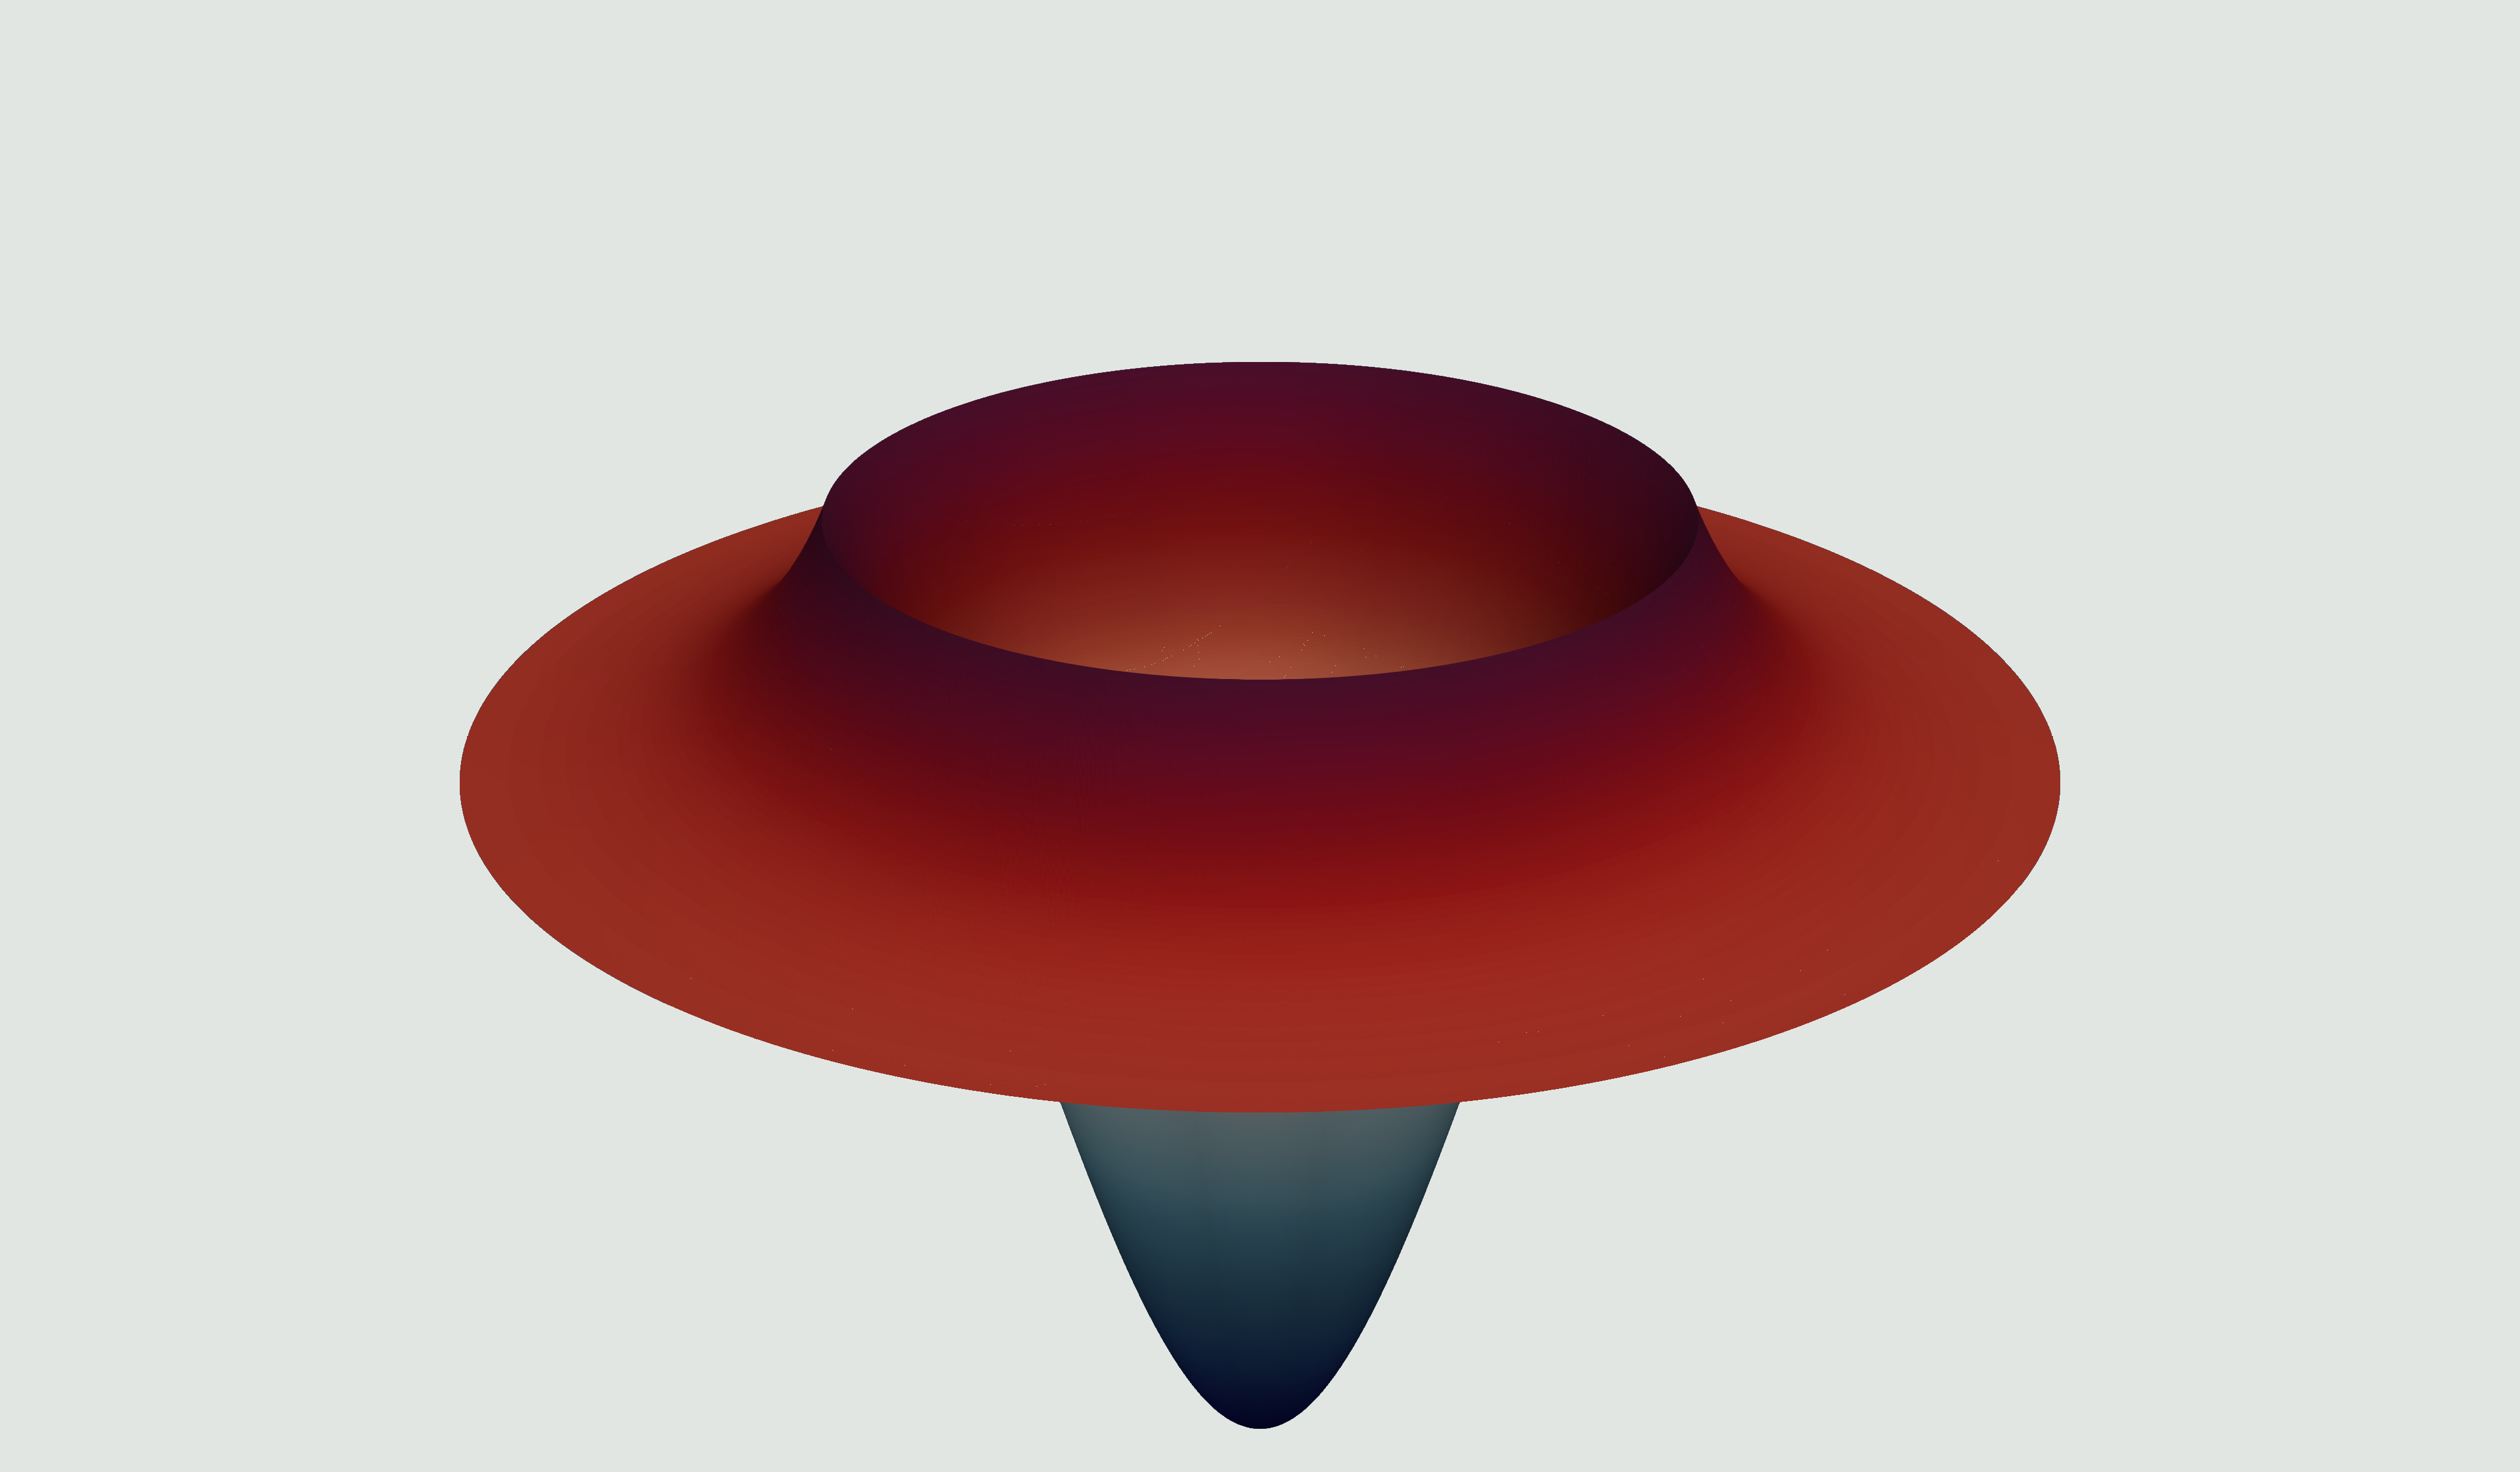
\includegraphics[width=0.49\textwidth]{images/ez2posterStepFiber.png}
	            \vspace{0.01\textwidth}
	            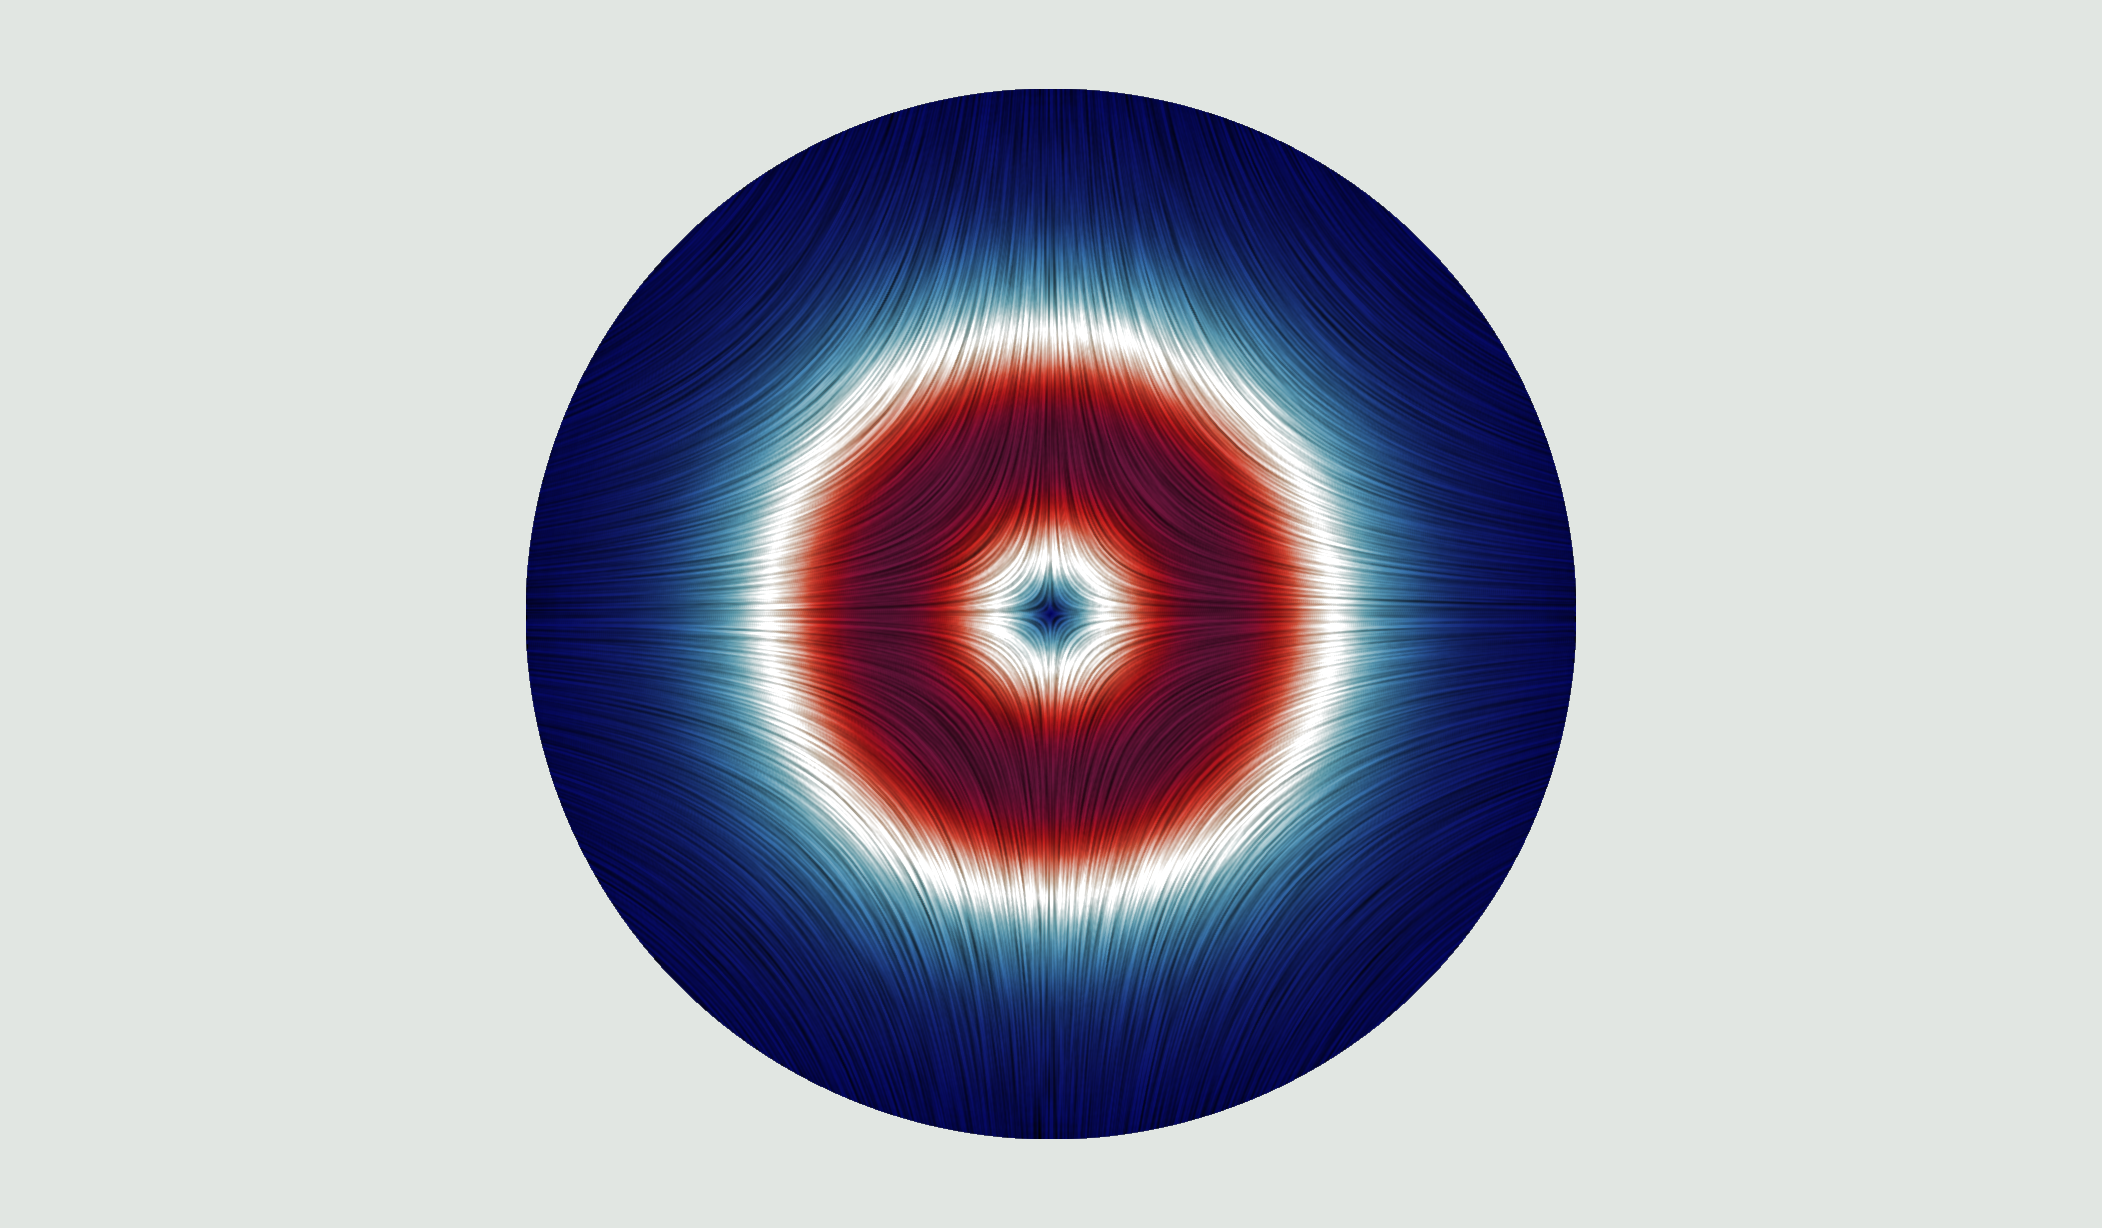
\includegraphics[width=0.49\textwidth]{images/et3posterStepFiber.png}%
	            \hspace{0.01\textwidth}%
	            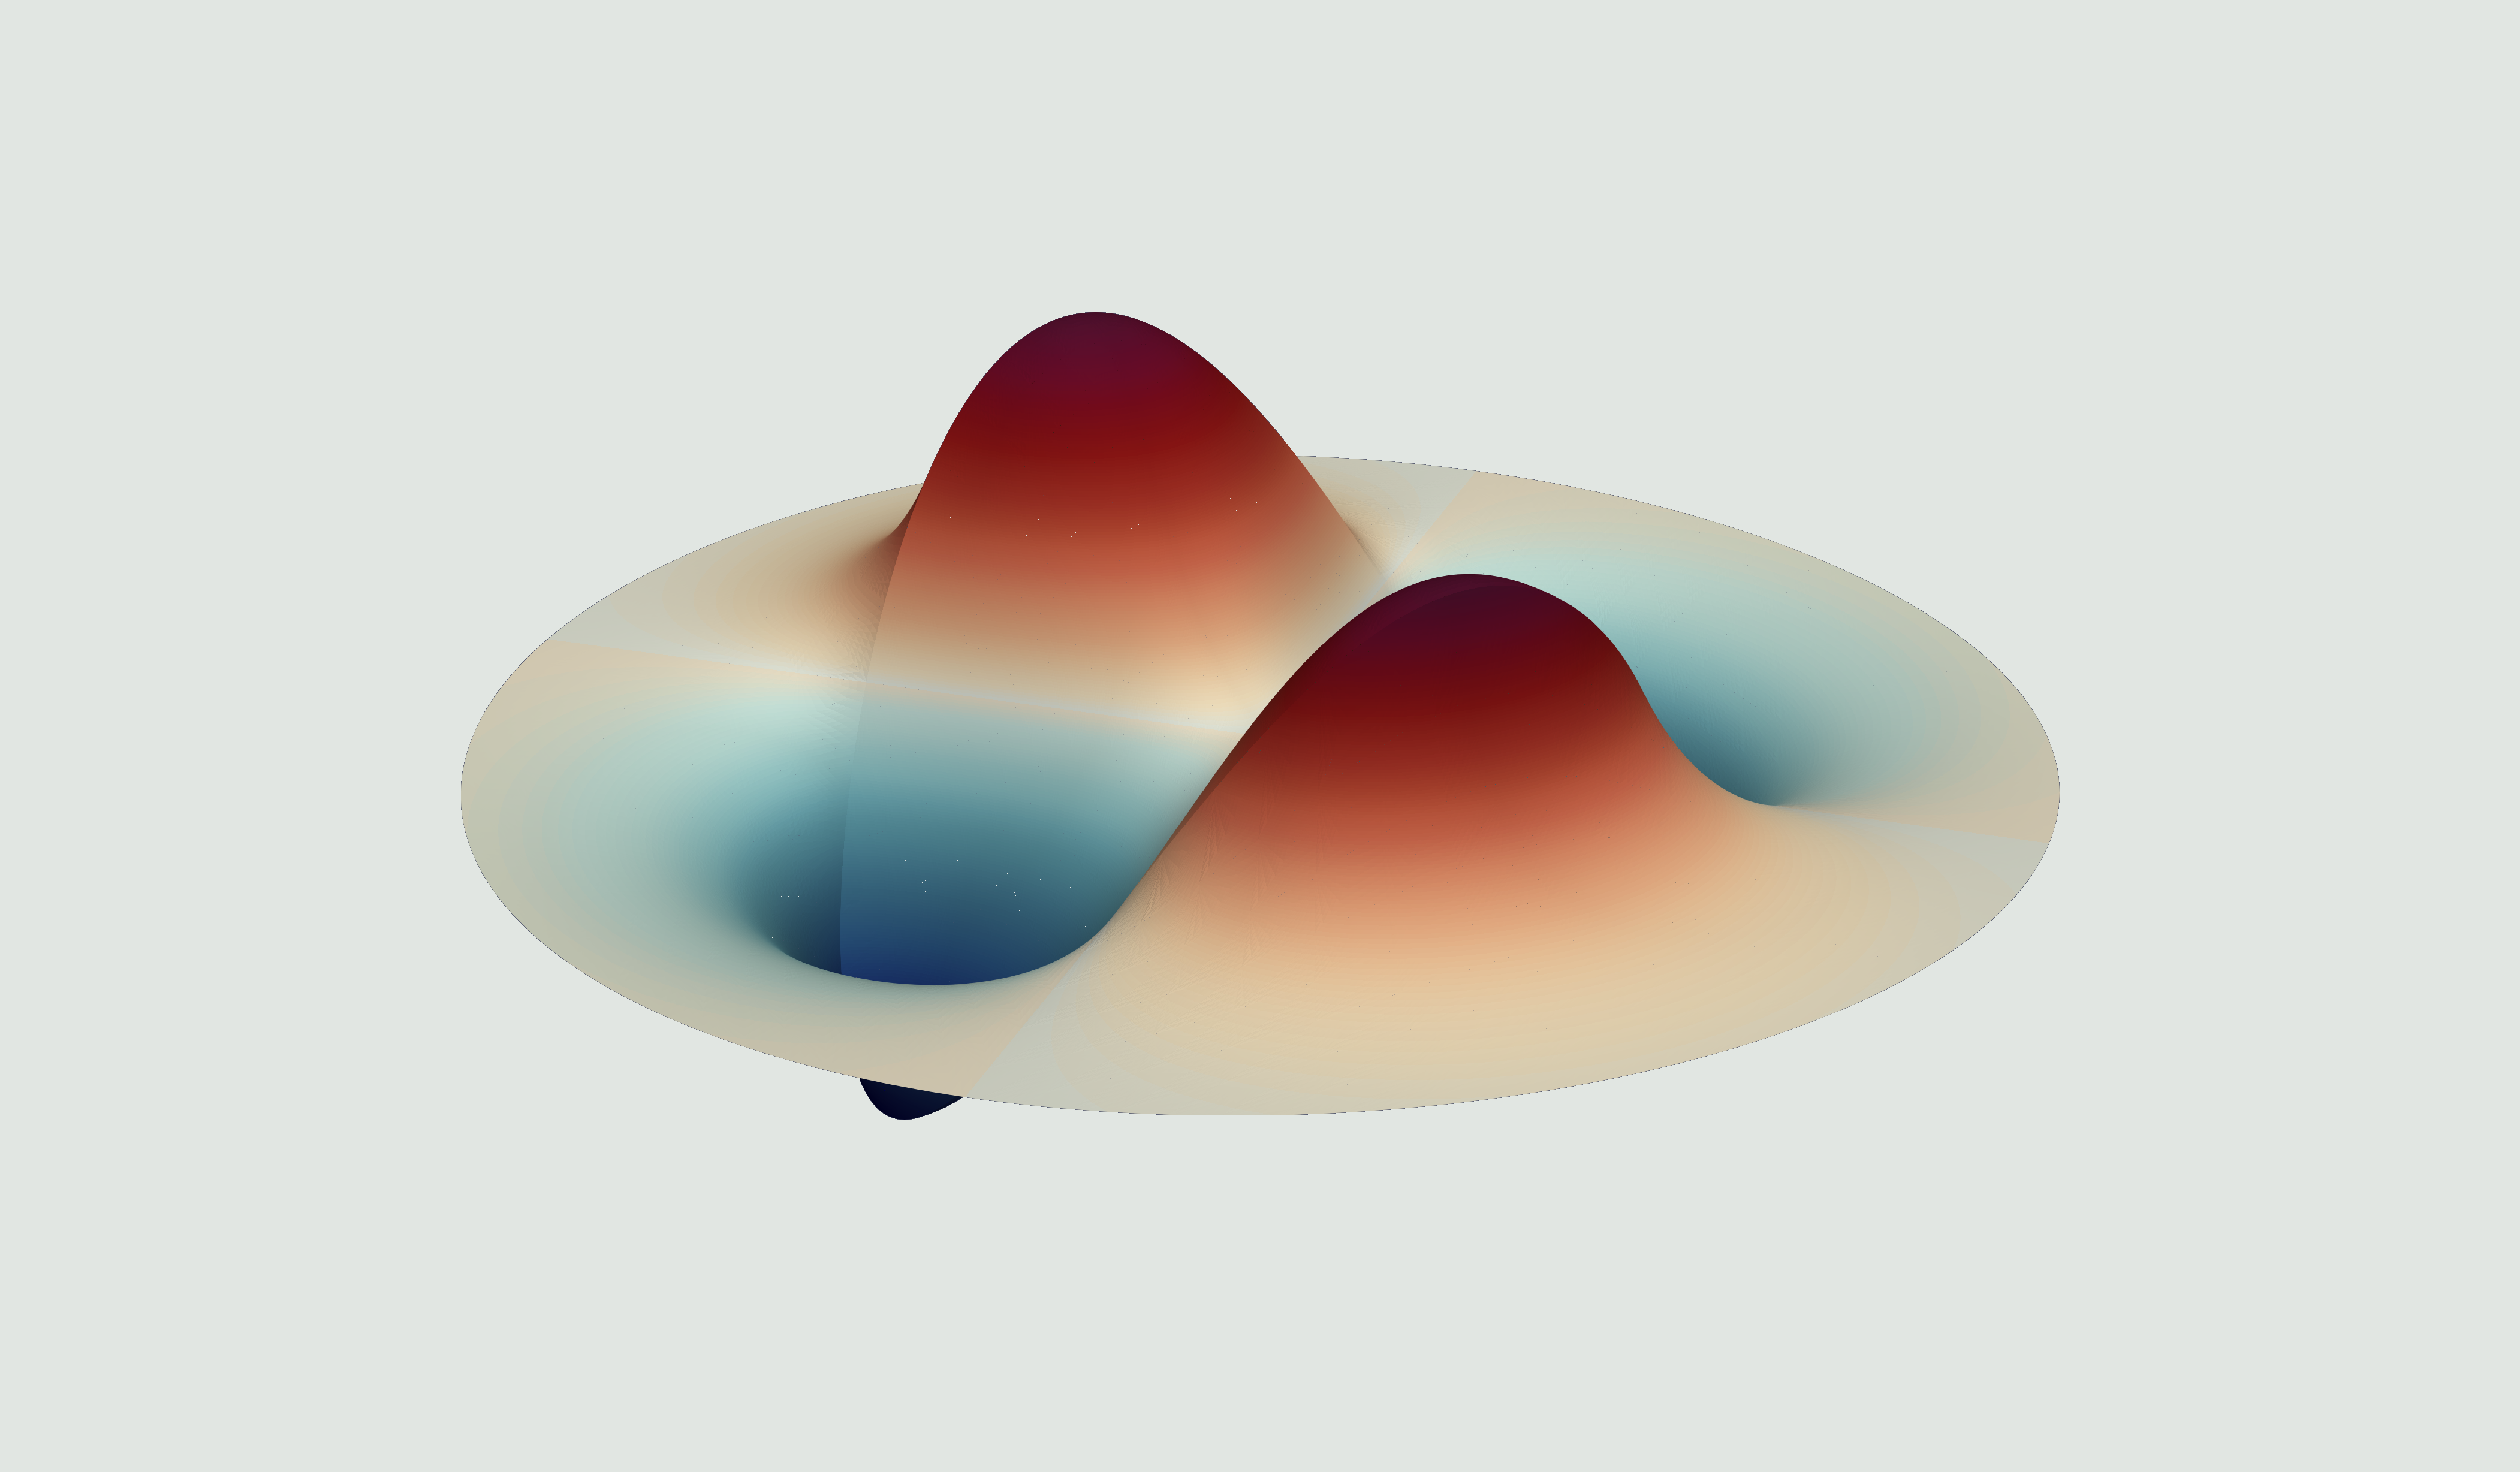
\includegraphics[width=0.49\textwidth]{images/ez3posterStepFiber.png}
	            \end{mdframed}
            \caption{BlaBlabla}
        \end{figure}
        \end{block}

        \vfill

      } % end of parbox
    \end{column}

    %% Right column:
    %% ============================================================
    \begin{column}{0.45\textwidth}
      \parbox[t][\columnheight]{\textwidth}{

        \vfill

        \begin{block}{\boxnumber HP-ADAPTIVITY CAPABILITIES }
        \begin{figure}
        	\centering
	            \begin{tikzpicture}%
	        		\node[anchor=south west, inner sep=0] (X) at (0,0){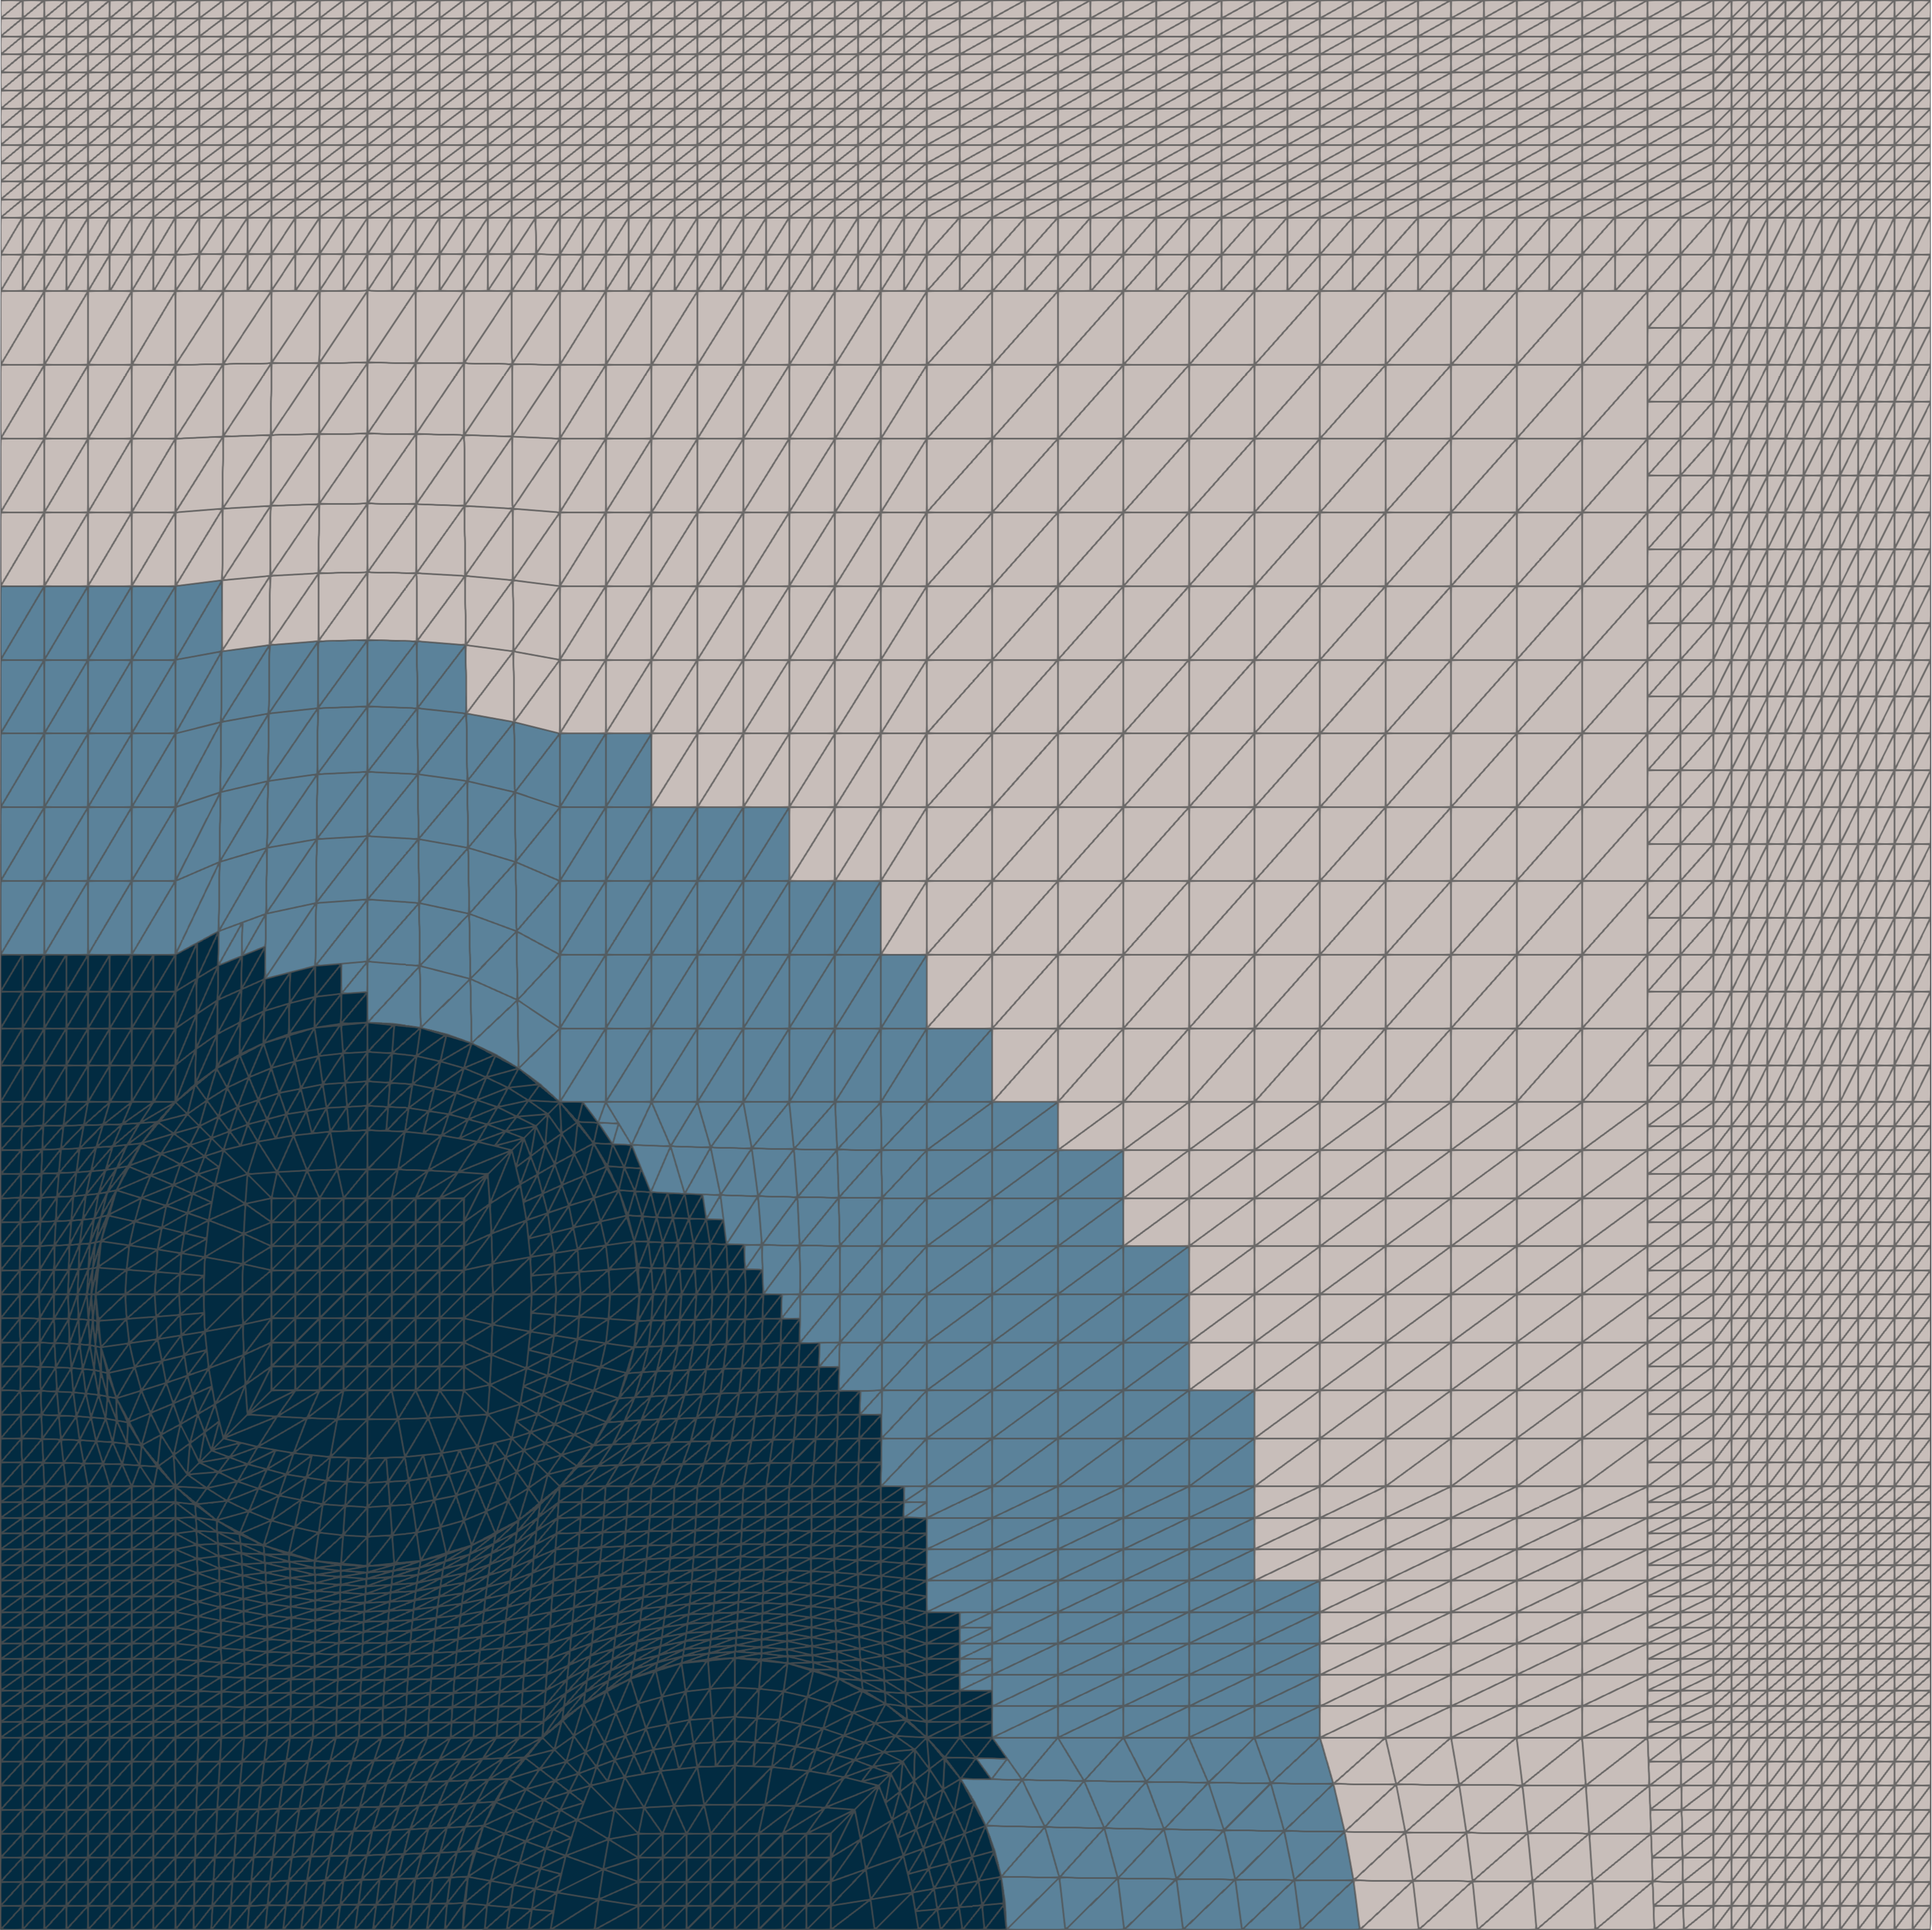
\includegraphics[height=0.8\linewidth]{images/holeyMesh.png}};%
	        		\begin{scope}[x={(X.south east)},y={(X.north west)}]%
	        		%% This makes all measurements with no units into fractions of the width
	        		%% and height of the graphic contained in the node.
	        		\draw[fill = white,fill opacity=0.8, text opacity=1] (0.05,0.075) rectangle (0.15,0.125) node[pos=.5] {$k=5$};
	        		\draw[fill = white,fill opacity=0.8, text opacity=1] (0.37,0.395) rectangle (0.47,0.445) node[pos=.5] {$k=4$};
	        		\draw[fill = white,fill opacity=0.8, text opacity=1] (0.65,0.675) rectangle (0.75,0.725) node[pos=.5] {$k=3$};
	        		\end{scope}%
	    	    \end{tikzpicture}
    	    \caption{Hello}
    	\end{figure}    	

    	\begin{figure}[hb]
	    	\begin{mdframed}[backgroundcolor=bggrey]
	            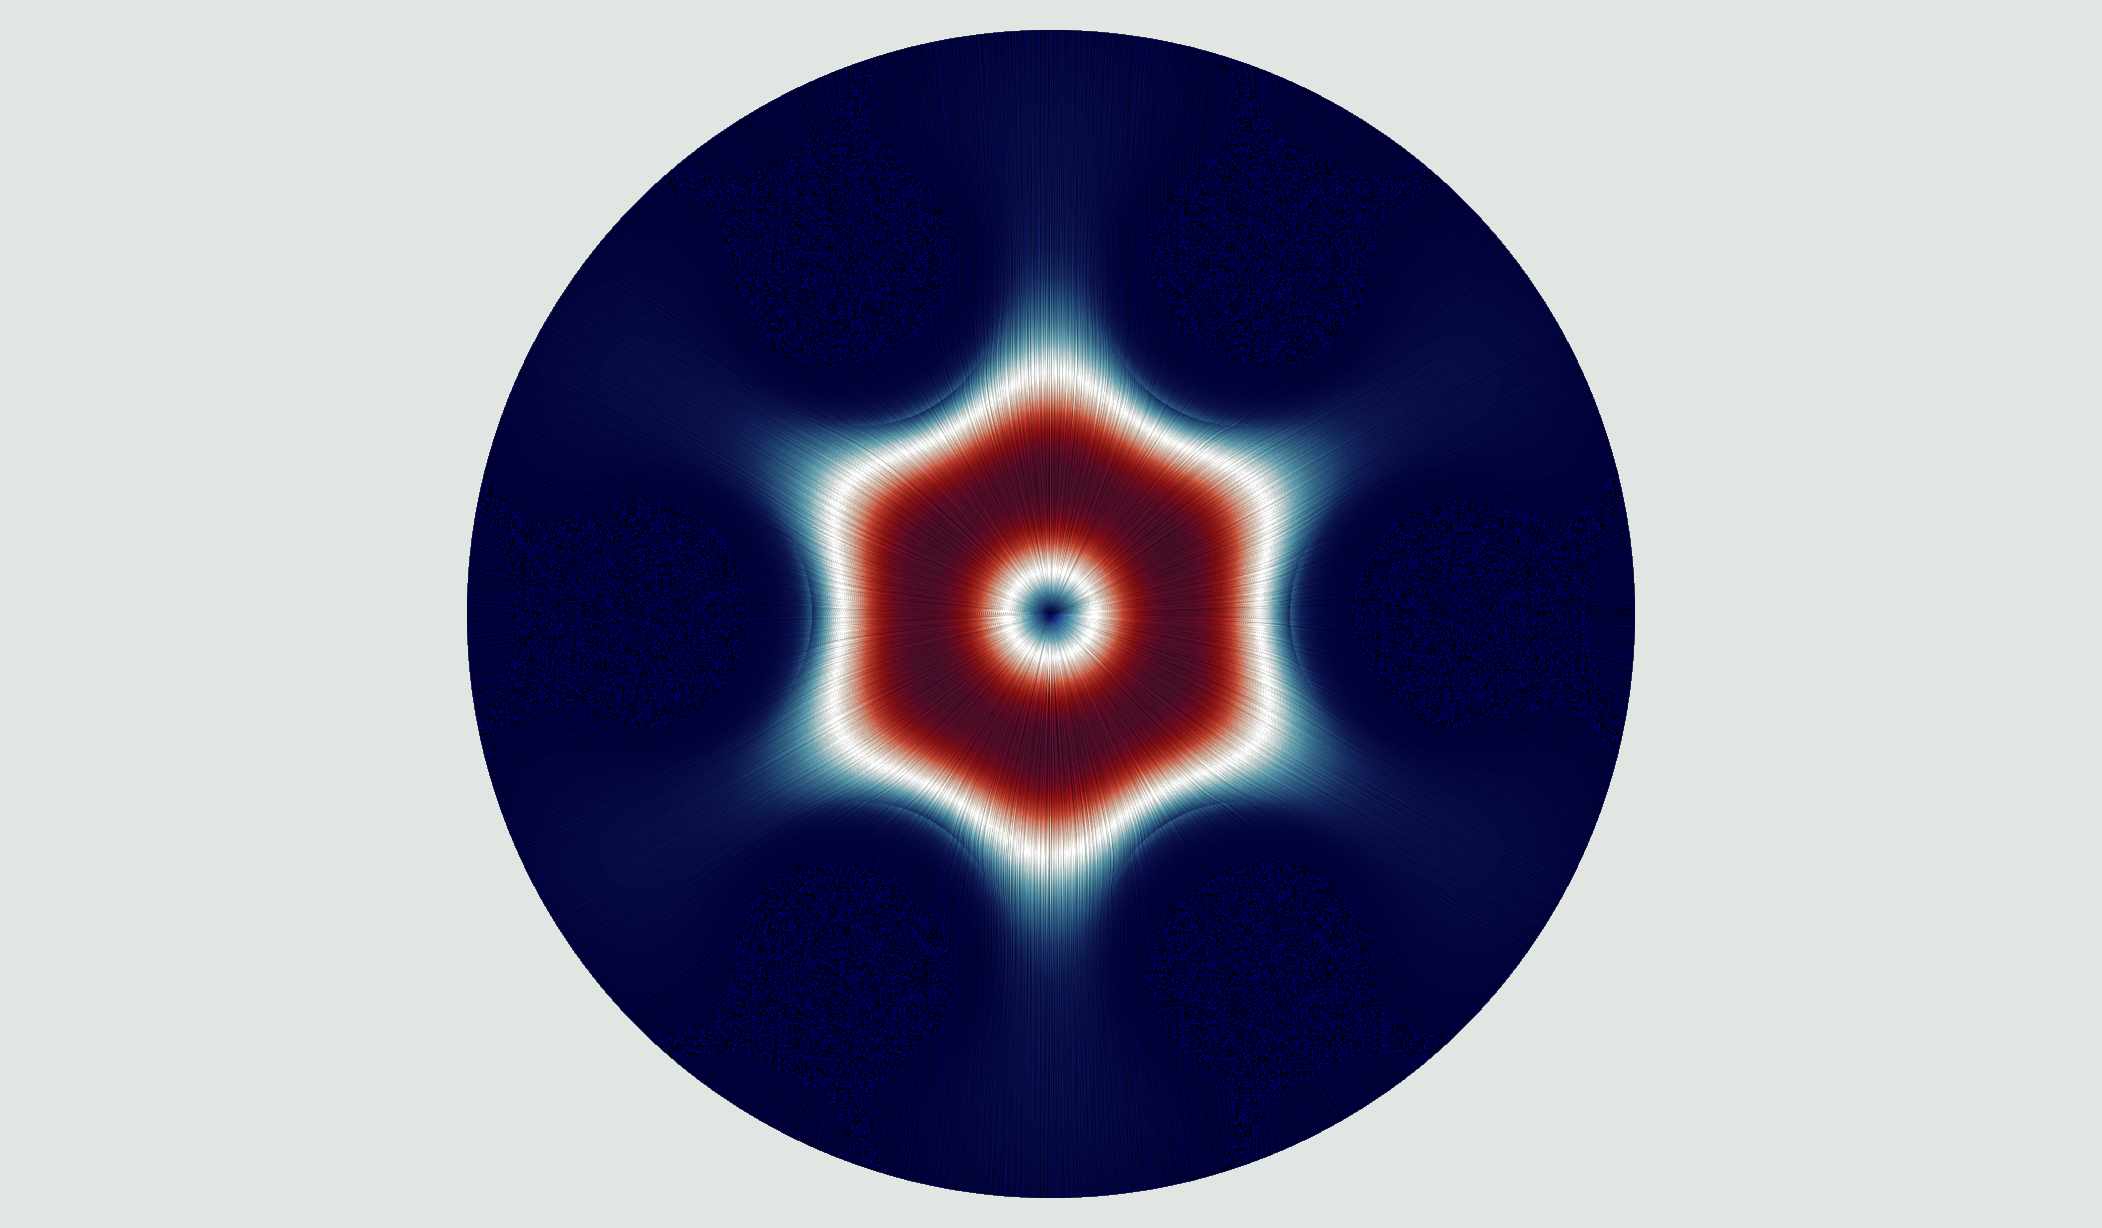
\includegraphics[width=0.49\textwidth]{images/et1posterHoley.png}%
	            \hspace{0.01\textwidth}%
	            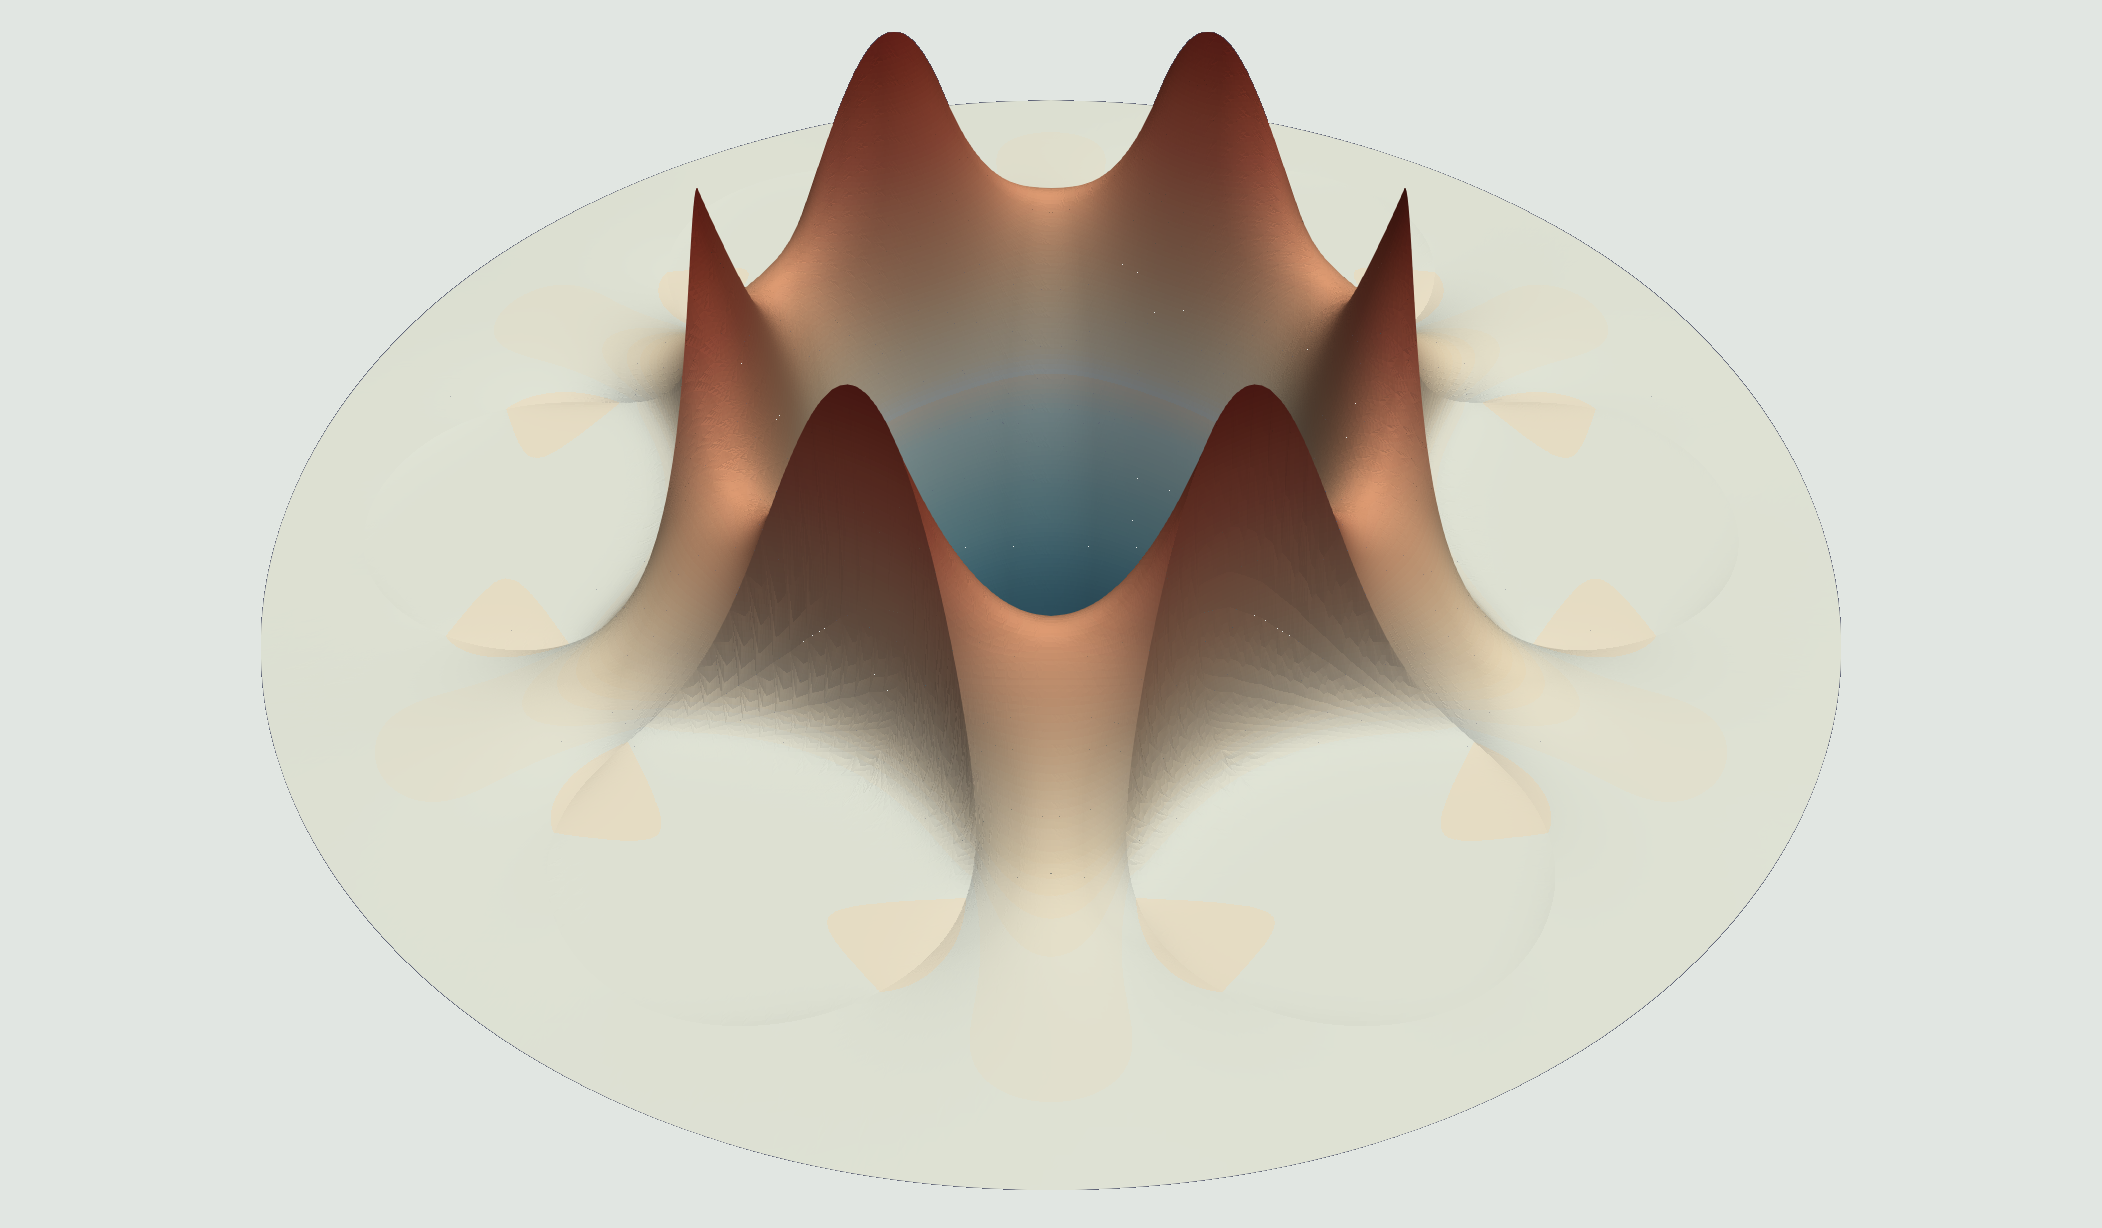
\includegraphics[width=0.49\textwidth]{images/ez1posterHoley.png}
	            \vspace{0.01\textwidth}
	            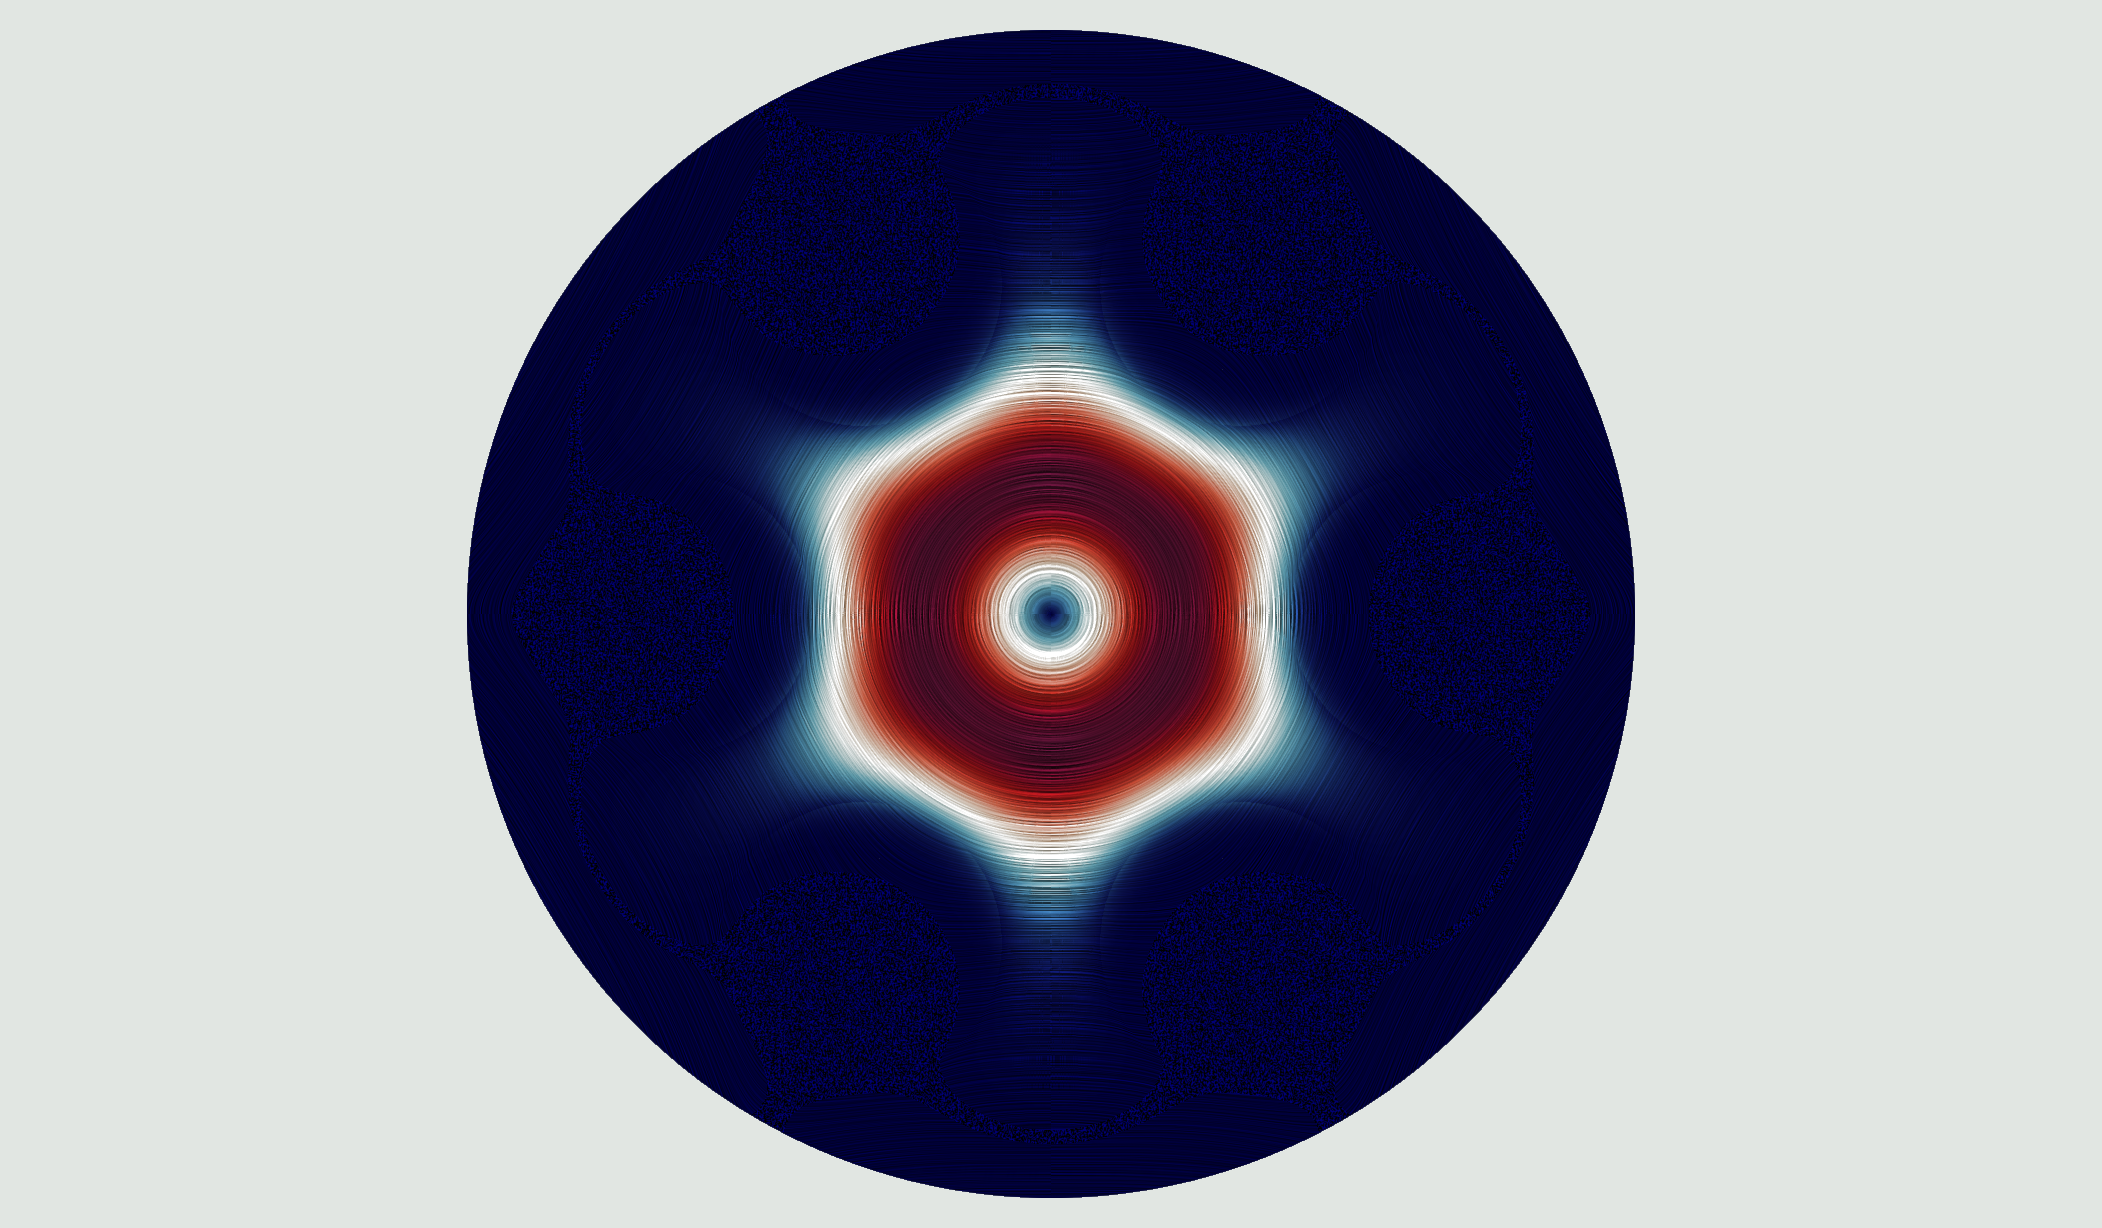
\includegraphics[width=0.49\textwidth]{images/et2posterHoley.png}%
	            \hspace{0.01\textwidth}%
	            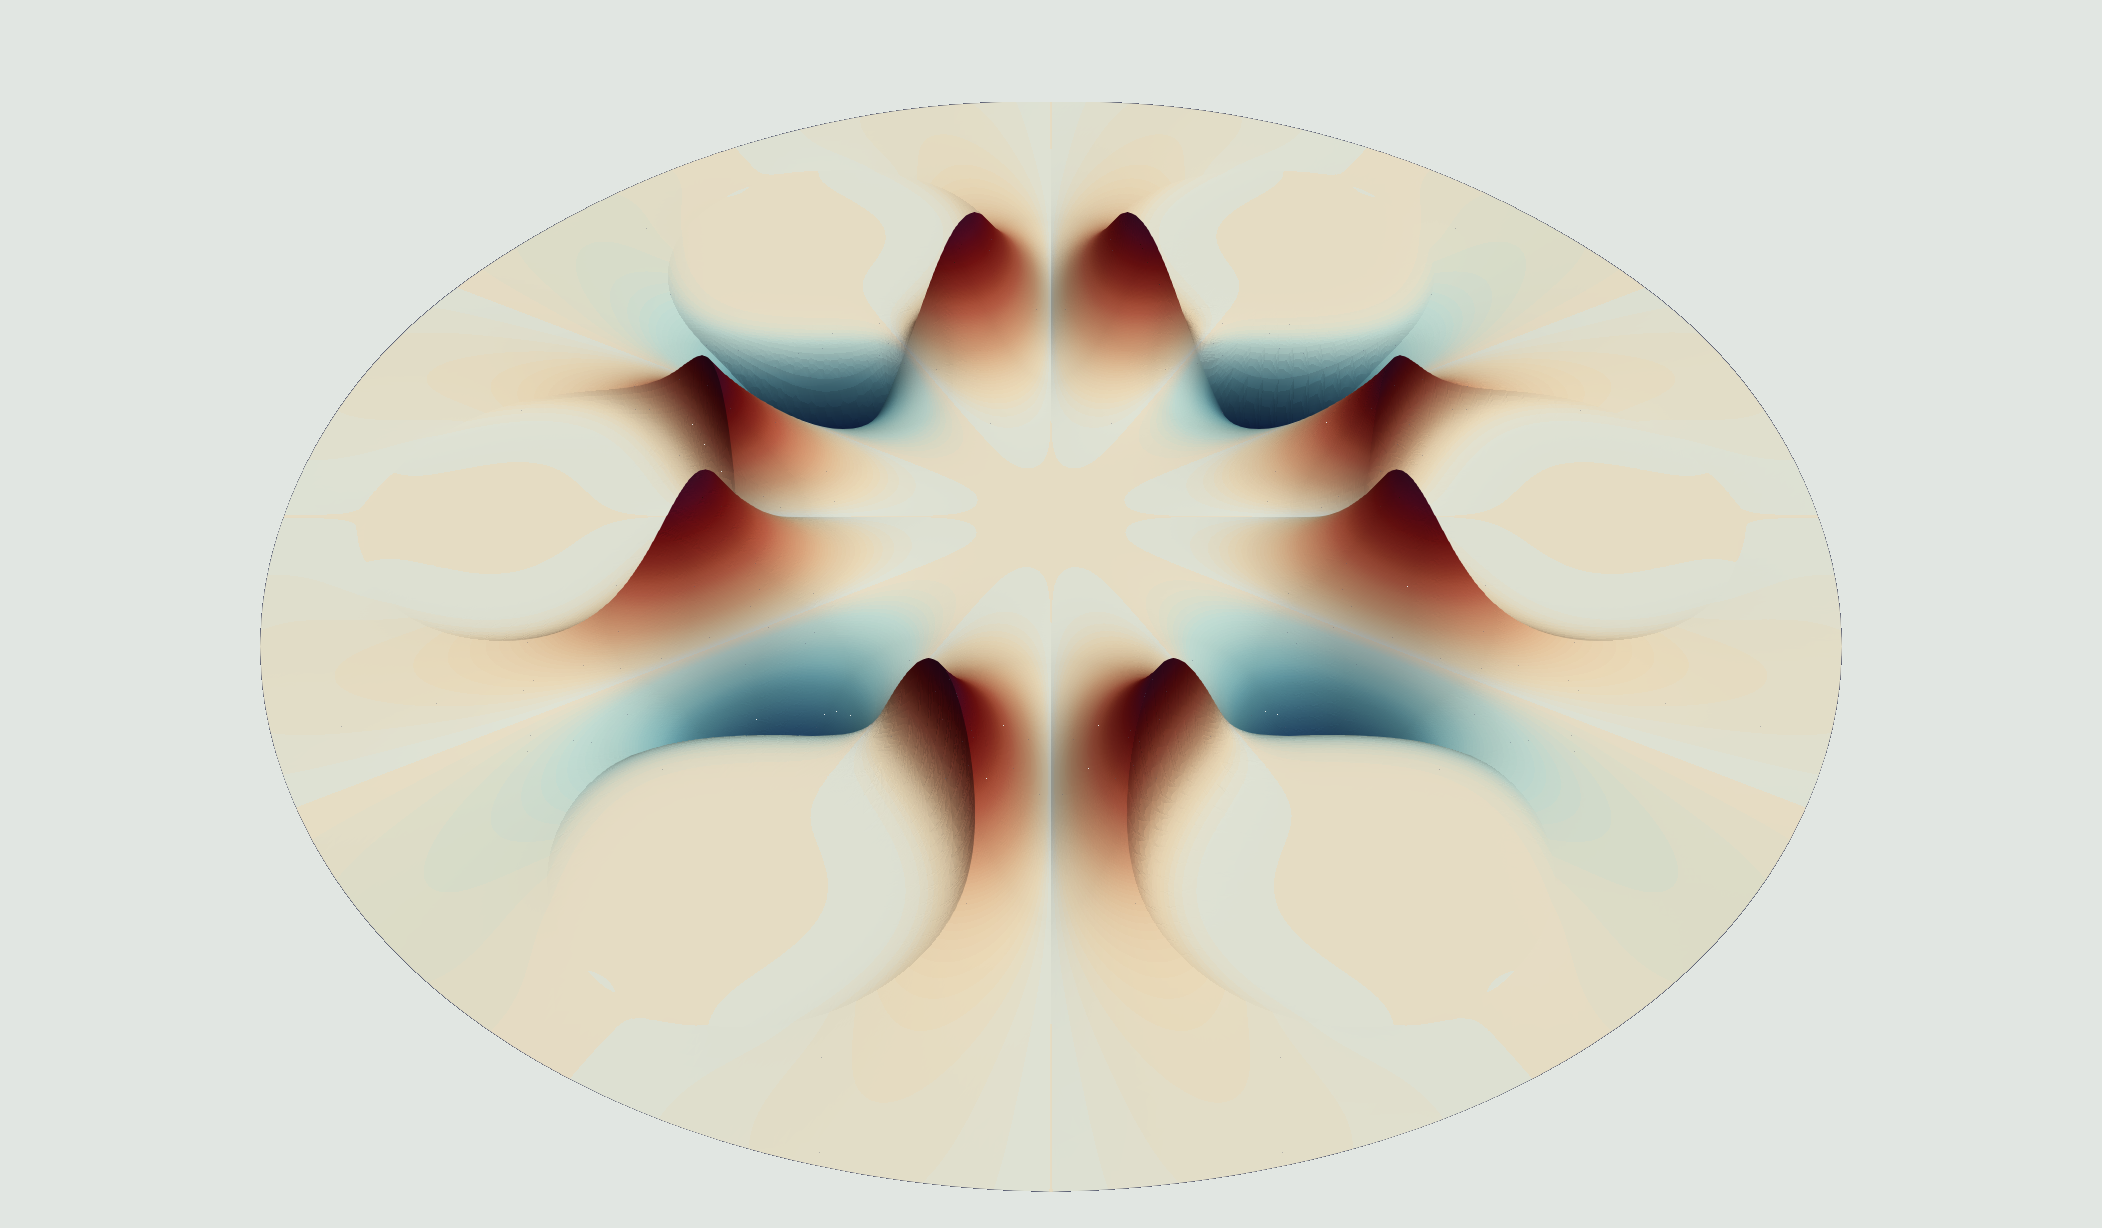
\includegraphics[width=0.49\textwidth]{images/ez2posterHoley.png}
	        \end{mdframed}
            \caption{BlaBlabla}
        \end{figure}
            % \begin{figure}[ht]
            %     \centering
            %     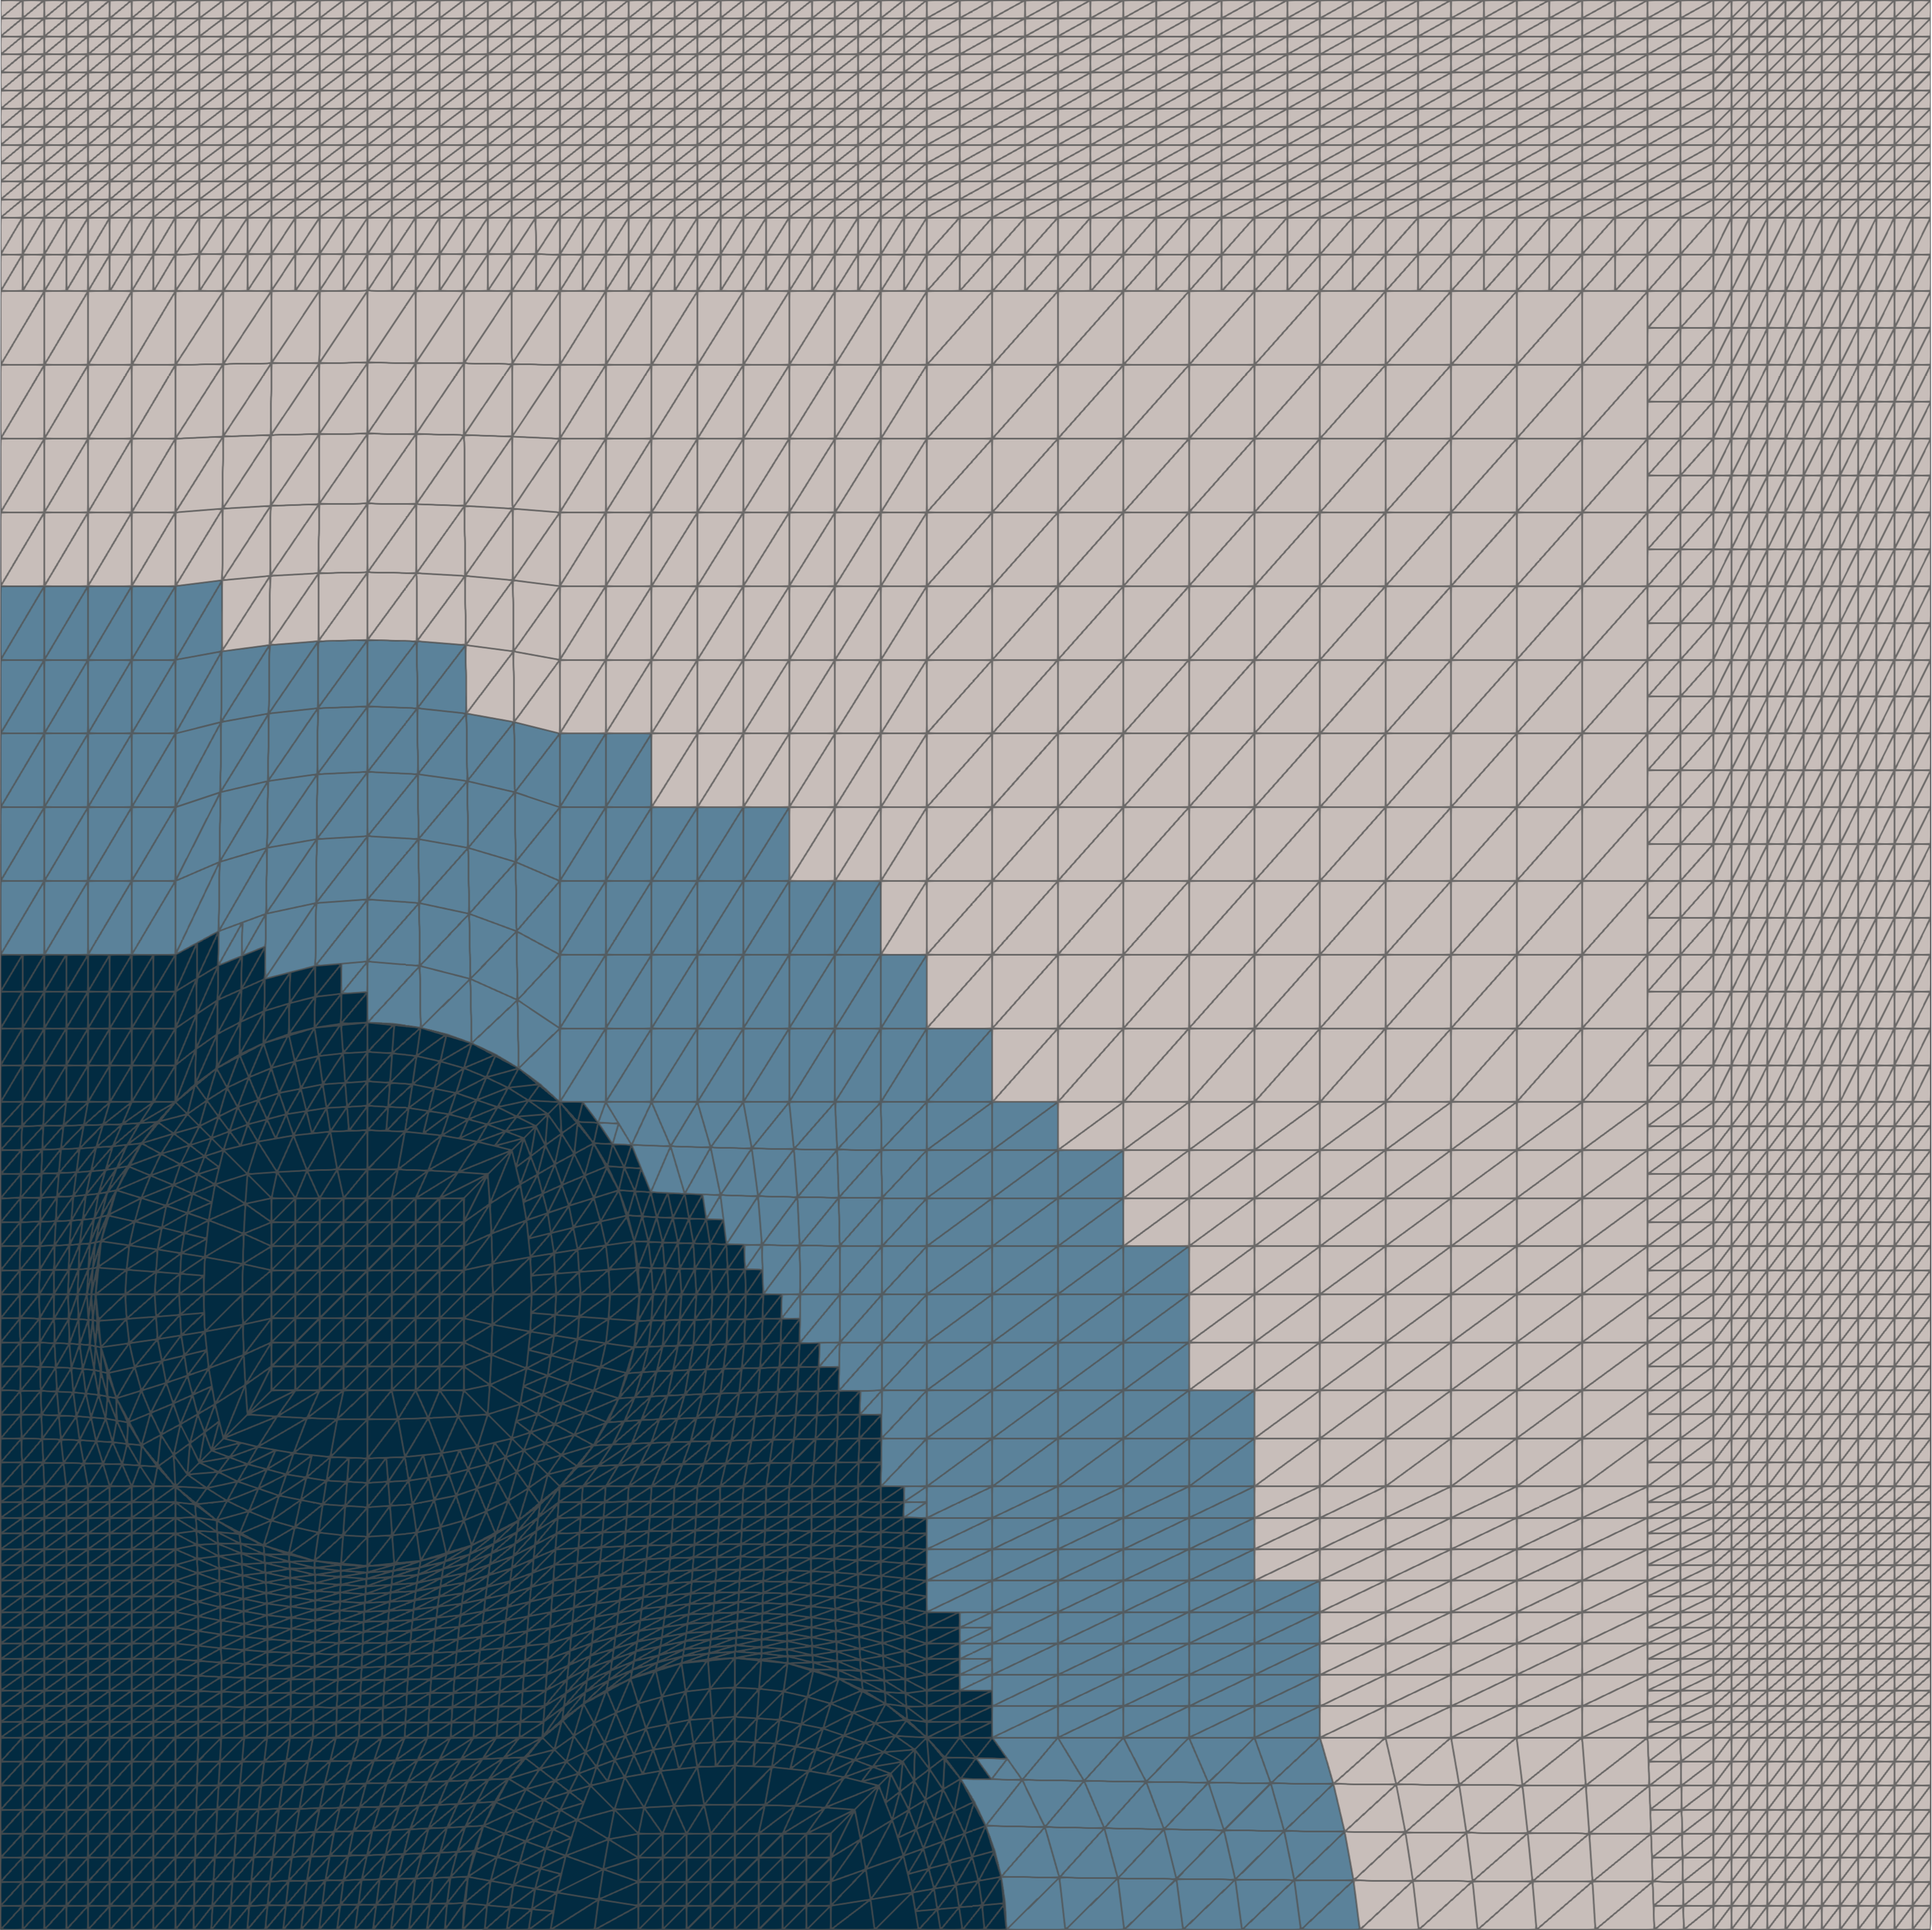
\includegraphics[width=1\linewidth]{images/holeyMesh.png}
            %     \caption{BlaBlabla}
            %     \label{fig:test2}
            % \end{figure}
        \end{block}

        \vfill

      } % end of parbox
    \end{column}

  \end{columns}
\end{frame}

\end{document}
